% needed by pyrepro manual section, which was converted by
% pandoc from markdown.
\providecommand{\tightlist}{%
  \setlength{\itemsep}{0pt}\setlength{\parskip}{0pt}}
\chapter{Interfaces}\label{interfaces}


\section{Overview}\label{interfaces:overview}

The \texttt{interface} specification in a Dakota input file controls
details of function evaluations. The mechanisms currently in place for
function evaluations involve interfacing with one or more
computational simulation codes, computing algebraic mappings (refer to
Section~\ref{advint:algebraic}), or a combination of the two.

%In the case of use of an approximation in place of an expensive
%simulation code, an \texttt{approximation} interface can be selected
%to make use of surrogate modeling capabilities available within
%Dakota.  Surrogate models are discussed further in Chapter~\ref{models}.

This chapter will focus on mechanisms for simulation code invocation,
starting with interface types in Section~\ref{interfaces:sim} and
followed by a guide to constructing simulation-based interfaces in
Section~\ref{interfaces:building}.  This chapter also provides an
overview of simulation interface components, covers issues relating to
file management, and presents a number of example data mappings.

For a detailed description of interface specification syntax, refer to
the interface commands chapter in the Dakota Reference Manual~\cite{RefMan}.


\section{Simulation Interfaces}\label{interfaces:sim}

The invocation of a simulation code is performed using either system
calls or forks or via direct linkage. In the system call and fork
cases, a separate process is created for the simulation and
communication between Dakota and the simulation occurs through
parameter and response files. For system call and fork interfaces, the
interface section must specify the details of this data transfer.  In
the direct case, a separate process is not created and communication
occurs in memory through a prescribed API.
Sections~\ref{interfaces:direct} through \ref{interfaces:which}
provide information on the simulation interfacing approaches.

\subsection{Direct Simulation Interface}\label{interfaces:direct}

The direct interface may be used to invoke
simulations that are linked into the Dakota executable. This
interface eliminates overhead from process creation and file I/O and
can simplify operations on massively parallel computers. These
advantages are balanced with the practicality of converting an
existing simulation code into a library with a subroutine
interface. Sandia codes for structural dynamics (Salinas),
computational fluid dynamics (Sage), and circuit simulation (Xyce) and
external codes such as Phoenix Integration's ModelCenter framework and
The Mathworks' Matlab have been linked in this way, and a direct
interface to Sandia's SIERRA multiphysics framework is under
development. In the latter case, the additional effort is particularly
justified since SIERRA unifies an entire suite of physics codes.
[\emph{Note: the ``sandwich implementation'' of combining a direct
interface plug-in with Dakota's library mode is discussed in the
Dakota Developers Manual~\cite{DevMan}}].

In addition to direct linking with simulation codes, the direct
interface also provides access to internal polynomial test functions
that are used for algorithm performance and regression testing. The
following test functions are available: \texttt{cantilever},
\texttt{cyl\_head}, \texttt{log\_ratio}, \texttt{rosenbrock},
\texttt{short\_column}, and \texttt{text\_book} (including
\texttt{text\_book1}, \texttt{text\_book2}, \texttt{text\_book3}, and
\texttt{text\_book\_ouu}). While these functions are also available
as external programs in the \path{dakota/share/dakota/test} directory,
maintaining internally linked versions allows more rapid testing. See
Chapter~\ref{additional} for additional information on several of
these test problems. An example input specification for a direct
interface follows:
\begin{small}
\begin{verbatim}
    interface,
            direct
              analysis_driver = 'rosenbrock'
\end{verbatim}
\end{small}

Additional specification examples are provided in
Section~\ref{tutorial:examples} and additional information on
asynchronous usage of the direct function interface is provided in
Section~\ref{parallel:SLP:local:direct}.  Guidance for usage of some
particular direct simulation interfaces is in
Section~\ref{advint:existingdirect} and the details of adding a
simulation code to the direct interface are provided in
Section~\ref{advint:direct}.

\subsection{System Call Simulation Interface}\label{interfaces:system}

{\bf Users are strongly encouraged to use the fork simulation
  interface if possible, though the system interface is still
  supported for portability and backward compatibility.}  The system
call approach invokes a simulation code or simulation driver by using
the \texttt{system} function from the standard C
library~\cite{Ker88}. In this approach, the system call creates a new
process that communicates with Dakota through parameter and response
files.  The system call approach allows the simulation to be initiated
via its standard invocation procedure (as a ``black box'') and then
coordinated with a variety of tools for pre- and post-processing.
This approach has been widely used in previous
studies~\cite{Eld96a,Eld96b,Eld98b}. The system call approach involves
more process creation and file I/O overhead than the direct function
approach, but this extra overhead is usually insignificant compared
with the cost of a simulation.  An example of a system call interface
specification follows:
\begin{small}
\begin{verbatim}
    interface,
            system
              analysis_driver = 'text_book'
              parameters_file = 'text_book.in'
              results_file    = 'text_book.out'
              file_tag file_save
\end{verbatim}
\end{small}

Information on asynchronous usage of the system interface is provided in
Section~\ref{parallel:SLP:local:system}.

\subsection{Fork Simulation Interface}\label{interfaces:fork}

The fork simulation interface uses the \texttt{fork}, \texttt{exec},
and \texttt{wait} families of functions to manage simulation codes or
simulation drivers. (In a native MS Windows version of Dakota, similar
Win32 functions, such as \texttt{\_spawnvp()}, are used instead.)
Calls to \texttt{fork} or \texttt{vfork} create a
copy of the Dakota process, \texttt{execvp} replaces this copy with
the simulation code or driver process, and then Dakota uses the
\texttt{wait} or \texttt{waitpid} functions to wait for completion of
the new process. Transfer of variables and response data between
Dakota and the simulator code or driver occurs through the file system
in exactly the same manner as for the system call interface. An
example of a fork interface specification follows:
\begin{small}
\begin{verbatim}
    interface,
            fork
              input_filter    = 'test_3pc_if'
              output_filter   = 'test_3pc_of'
              analysis_driver = 'test_3pc_ac'
              parameters_file = 'tb.in'
              results_file    = 'tb.out'
              file_tag
\end{verbatim}
\end{small}

More detailed examples of using the fork call interface are provided
in Section~\ref{tutorial:examples:user_supply:optimization1} and in
Section~\ref{interfaces:building}, and information on asynchronous usage
of the fork call interface is provided in
Section~\ref{parallel:SLP:local:fork}.


\subsection{Syntax for Filter and Driver Strings}\label{interfaces:syntax}

Dakota's default behavior is to construct input filter, analysis driver, and
output filter commands by appending the names of the parameters file and results file
for the evaluation/analysis to the user-provided
\texttt{input\_filter}, \texttt{output\_filter}, and \texttt{analysis\_drivers} 
strings. After adding its working directory to the \texttt{PATH}, Dakota executes 
these commands in its working directory or, if the \texttt{work\_directory} keyword 
group is present, in a work directory.

Filter and driver strings may contain absolute or relative path information and 
whitespace; Dakota will pass them through without modification.

Quotes are also permitted with the restriction that if double-quotes (") are used to 
enclose the driver or filter string as a whole, then only single quotes (') are allowed 
within it, and vice versa. The input filter string \texttt{'dprepro --var "foo=1"'} 
works, as does \texttt{"dprepro --var 'foo=1'"}, but not \texttt{"dprepro --var "foo=1""}.

In some situations, users may not wish Dakota to append the names of the parameters
or results files to filter and driver strings. The \texttt{verbatim} keyword prevents
this behavior, and causes Dakota to execute filter and driver strings "as is".

Beginning with version 6.10, Dakota will substitute the tokens \texttt{\{PARAMETERS\}} 
and \texttt{\{RESULTS\}} in driver and filter strings with the names of the parameters 
and results files for that analysis/evaluation just prior to execution.

For example, if an \texttt{interface} block in the input file included:

\begin{verbatim}
  input_filter 'preprocess {PARAMETERS}'
  analysis_drivers 'run_sim.sh'
  output_filter 'postprocess {RESULTS}'
  verbatim
\end{verbatim}

Then, the input filter \texttt{preprocess} would be run with only the parameters file 
as a command line argument, the analysis driver \texttt{run\_sim.sh} would receive no 
command line arguments, and the output filter \texttt{postprocess} would receive only 
the results file name.

The combination of \texttt{verbatim} and substitution provide users with considerable
flexibility in specifying the form of filter and driver commands.

\subsection{Fork or System Call: Which to Use?}\label{interfaces:which}

The primary operational difference between the fork and system call
simulation interfaces is that, in the fork interface, the
\texttt{fork}/\texttt{exec} functions return a process identifier
that the \texttt{wait}/\texttt{waitpid} functions can use
to detect the completion of a simulation for either synchronous or
asynchronous operations.  The system call simulation interface, on the
other hand, must use a response file detection scheme for this purpose
in the asynchronous case. Thus, an important advantage of the fork
interface over the system call interface is that it avoids the
potential of a file race condition when employing asynchronous local
parallelism (refer to Section~\ref{parallel:SLP:local}). This condition
can occur when the responses file has been created but the writing of
the response data set to this file has not been completed (see
Section~\ref{parallel:SLP:local:system}). While significant care has been
taken to manage this file race condition in the system call case, the
fork interface still has the potential to be more robust when
performing function evaluations asynchronously.

Another advantage of the fork interface is that it has additional
asynchronous capabilities when a function evaluation involves multiple
analyses. As shown in Table~\ref{parallel:table01}, the fork interface
supports asynchronous local and hybrid parallelism modes for managing
concurrent analyses within function evaluations, whereas the system
call interface does not. These additional capabilities again stem from
the ability to track child processes by their process
identifiers.

The only disadvantage to the fork interface compared with
the system interface is that the
\texttt{fork}/\texttt{exec}/\texttt{wait} functions are not part of
the standard C library, whereas the \texttt{system} function is. As a
result, support for implementations of the
\texttt{fork}/\texttt{exec}/\texttt{wait} functions can vary from
platform to platform. At one time, these commands were not available
on some of Sandia's massively parallel computers. However, in the more
mainstream UNIX environments, availability of
\texttt{fork}/\texttt{exec}/\texttt{wait} should not be an issue.

In summary, the system call interface has been a workhorse for many
years and is well tested and proven, but the fork interface
supports additional capabilities and is recommended when managing
asynchronous simulation code executions. Having both interfaces
available has proven to be useful on a number of occasions and they
will both continue to be supported for the foreseeable future.


\section{Building a Black-Box Interface to a Simulation Code}\label{interfaces:building}

To interface a simulation code to Dakota using one of the black-box
interfaces (system call or fork), pre- and post-processing
functionality typically needs to be supplied (or developed) in order
to transfer the parameters from Dakota to the simulator input file and
to extract the response values of interest from the simulator's output
file for return to Dakota (see Figures~\ref{intro:bbinterface}
and~\ref{interfaces:bbinterfacecomp}). This is often managed through
the use of scripting languages, such as C-shell~\cite{And86}, Bourne
shell~\cite{Bli96}, Perl~\cite{Wal96}, or Python~\cite{Mar03}. While
these are common and convenient choices for simulation
drivers/filters, it is important to recognize that any executable file
can be used. If the user prefers, the desired pre- and post-processing
functionality may also be compiled or interpreted from any number of
programming languages (C, C++, F77, F95, JAVA, Basic, etc.).

In the \path{dakota/share/dakota/examples/official/drivers/bash/} directory,
a simple example uses the Rosenbrock test function as a mock
engineering simulation code. Several scripts have been included to
demonstrate ways to accomplish the pre- and post-processing
needs. Actual simulation codes will, of course, have different pre-
and post-processing requirements, and as such, this example serves
only to demonstrate the issues associated with interfacing a
simulator. Modifications will almost surely be required for new
applications.

\subsection{Generic Script Interface Files}\label{interfaces:generic}

The \path{dakota/share/dakota/examples/official/drivers/bash/}
directory contains four important files:
\path{dakota_rosenbrock.in} (the Dakota input file),
\path{simulator_script.sh} (the simulation driver script),
\path{templatedir/ros.template} (a template simulation input file), and
\path{templatedir/rosenbrock_bb.py} (the Rosenbrock simulator).

The file \path{dakota_rosenbrock.in} specifies the study that
Dakota will perform and, in the interface section, describes the
components to be used in performing function evaluations. In
particular, it identifies \path{simulator_script.sh} as its
\texttt{analysis\_driver}, as shown in Figure~\ref{advint:figure01}.
\begin{figure}
  \centering
  \begin{bigbox}
    \begin{small}
      \verbatimtabinput[8]{dakota_rosenbrock.in}
    \end{small}
  \end{bigbox}
  \caption{The \protect\path{dakota_rosenbrock.in} input file.}
  \label{advint:figure01}
\end{figure}

The \path{simulator_script.sh} listed in Figure~\ref{advint:figure02}
is a short driver shell script that Dakota executes to perform each
function evaluation. The names of the parameters and results files are
passed to the script on its command line; they are
referenced in the script by \texttt{\$1}
and \texttt{\$2}, respectively. The \path{simulator_script.sh}
is divided into three parts: pre-processing, analysis, and post-processing.
% is divided into five parts: set up, pre-processing, analysis,
% post-processing, and clean up.

\begin{figure}
  \centering
  \begin{bigbox}
    \begin{small}
      \verbatimtabinput[8]{simulator_script.sh}
    \end{small}
  \end{bigbox}
  \caption{The \protect\path{simulator_script.sh} sample driver script.}
  \label{advint:figure02}
\end{figure}

In the pre-processing portion, the \path{simulator_script.sh} uses
\path{dprepro}, a template processing utility, to extract the
current variable values from a parameters file (\texttt{\$1})
and combine them with the simulator template input file
(\path{ros.template}) to create a new input file (\path{ros.in})
for the simulator. Internal to Sandia, the APREPRO utility is often
used for this purpose. For external sites where APREPRO is not
available, \texttt{dprepro} is an alternative with many of the 
capabilities of APREPRO that is specifically tailored for use with Dakota
and is distributed with it (in \path{dakota/scripts/pyprepro/}, or
\path{dakota/bin} in a binary distribution). Dakota also provides a second,
more general-purpose template processing tool named \texttt{pyprepro}, 
which is as a Python-based alternative to APREPRO. This pair of
tools, which permit not only parameter substitution, but execution of
arbitrary Python scripting within templates, is extensively documented in 
Section~\ref{interfaces:dprepro-and-pyprepro}.

Other preprocessing tools of potential interest are the BPREPRO
utility (see~\cite{WalXX}), and at Lockheed Martin sites, the JPrePost 
utility, a JAVA pre- and post-processor~\cite{Fla}. The \texttt{dprepro} script
will be used here for simplicity of discussion. It can use either 
Dakota's \texttt{aprepro} parameters file format (see
Section~\ref{variables:parameters:aprepro}) or Dakota's standard
format (see Section~\ref{variables:parameters:standard}), so either
option may be selected in the interface section of the Dakota input
file. The \path{ros.template} file listed in
Figure~\ref{advint:figure04} is a template simulation input file which
contains targets for the incoming variable values, identified by the
strings ``\texttt{\{x1\}}'' and ``\texttt{\{x2\}}''. These
identifiers match the variable descriptors specified in
\path{dakota_rosenbrock.in}. The template input file is contrived
as Rosenbrock has nothing to do with finite element analysis; it only
mimics a finite element code to demonstrate the simulator
template process. The \texttt{dprepro} script will search the
simulator template input file for fields marked with curly
brackets and then create a new file (\path{ros.in}) by replacing
these targets with the corresponding numerical values for the
variables. As shown in \path{simulator_script.sh}, the names for the Dakota
parameters file (\texttt{\$1}), template file
(\path{ros.template}), and generated input file (\path{ros.in})
must be specified in the \texttt{dprepro} command line arguments.

\begin{figure}
  \centering
  \begin{bigbox}
    \begin{small}
      \verbatimtabinput[8]{ros.template}
    \end{small}
  \end{bigbox}
  \caption{Listing of the \protect\path{ros.template} file}
  \label{advint:figure04}
\end{figure}

The second part of the script executes the \path{rosenbrock_bb.py}
simulator. The input and output file names, \path{ros.in} and
\path{ros.out}, respectively, are hard-coded into the. When the 
\path{./rosenbrock_bb.py} simulator is executed, the values for \texttt{x1} 
and \texttt{x2} are read in from \path{ros.in}, the Rosenbrock function is evaluated,
and the function value is written out to \path{ros.out}.

The third part performs the post-processing and writes the response
results to a file for Dakota to read. Using the UNIX ``\texttt{grep}'' utility, the
particular response values of interest are extracted from the raw
simulator output and saved to a temporary file (\path{results.tmp}).
When complete, this file is renamed \texttt{\$2}, which in this
example is always ``\path{results.out}''.
Note that moving or renaming the completed results file
avoids any problems with read race
conditions (see Section~\ref{parallel:SLP:local:system}).

% Finally, in the clean up phase, the working directory is removed to
% reduce the amount of disk storage required to execute the study. If
% data from each simulation needs to be saved, this step can be
% commented out by inserting a ``\texttt{\#}'' character before
% ``\texttt{$\backslash$rm -rf}''.

Because the Dakota input file \path{dakota_rosenbrock.in}
(Figure~\ref{advint:figure01}) specifies
\texttt{work\_directory} and \texttt{directory\_tag} in its interface
section, each invocation of \path{simulator_script.sh} wakes up in
its own temporary directory, which Dakota has populated with the
contents of directory \path{templatedir/}. Having a separate directory
for each invocation of \path{simulator_script.sh} simplifies the script
when the Dakota input file specifies \texttt{asynchronous} (so
several instances of \path{simulator_script.sh} might run simultaneously),
as fixed names such as \path{ros.in}, \path{ros.out}, and \path{results.tmp}
can be used for intermediate files. If neither \texttt{asynchronous} nor
\texttt{file\_tag} is specified, and if there is no need (e.g., for debugging)
to retain intermediate files having fixed names, then \texttt{directory\_tag}
offers no benefit and can be omitted. An alternative to \texttt{directory\_tag}
is to proceed as earlier versions of this chapter --- prior to Dakota 5.0's
introduction of \texttt{work\_directory} --- recommended:  add two more
steps to the \path{simulator_script.sh},
an initial one to create a temporary directory explicitly and
copy \path{templatedir/} to it if needed, and a final step to remove the temporary
directory and any files in it.

When \texttt{work\_directory} is specified, Dakota adjusts the \texttt{\$PATH} seen
by \path{simulator_script.sh} so that simple program names
%in the \path{simulator_script}
(i.e., names not containing a slash) that
are visible in Dakota's directory will also be visible in the work directory.
Relative path names ---
involving an intermediate slash but not an initial one,
such as \path{./rosenbrock_bb.py} or \path{a/bc/rosenbrock_bb} ---
will only be visible in the work directory if a \texttt{link\_files}
or \texttt{copy\_files} specification (see \S\ref{interfaces:workdir})
has made them visible there.

As an example of the data flow on a particular function evaluation,
consider evaluation 60. The parameters file for this evaluation consists of:
\begin{small}
\begin{verbatim}
                                          2 variables
                      4.664752623441543e-01 x1
                      2.256400864298234e-01 x2
                                          1 functions
                                          3 ASV_1:obj_fn
                                          2 derivative_variables
                                          1 DVV_1:x1
                                          2 DVV_2:x2
                                          0 analysis_components
                                         60 eval_id
\end{verbatim}
\end{small}

This file is called \path{workdir/workdir.60/params.in} if the line
\begin{small}
\begin{verbatim}
 	  named 'workdir' file_save  directory_save
\end{verbatim}
\end{small}
in Figure~\ref{advint:figure01} is uncommented.
The first portion of the file indicates that there are two variables,
followed by new values for variables \texttt{x1} and \texttt{x2}, and
one response function (an objective function), followed by an active
set vector (ASV) value of \texttt{1}. The ASV indicates the need to
return the value of the objective function for these parameters (see
Section~\ref{variables:asv}). The \path{dprepro} script reads the
variable values from this file, namely \texttt{4.664752623441543e-01}
and \texttt{2.256400864298234e-01} for \texttt{x1} and \texttt{x2}
respectively, and substitutes them in the \texttt{\{x1\}} and
\texttt{\{x2\}} fields of the \path{ros.template} file. The final
three lines of the resulting input file (\path{ros.in}) then appear
as follows:
\begin{small}
\begin{verbatim}
variable 1 0.4664752623
variable 2 0.2256400864
end
\end{verbatim}
\end{small}

where all other lines are identical to the template file. The
\path{rosenbrock_bb} simulator accepts \path{ros.in} as its input
file and generates the following output to the file \path{ros.out}:
\begin{small}
\begin{verbatim}
 Beginning execution of model: Rosenbrock black box
 Set up complete.
 Reading nodes.
 Reading elements.
 Reading materials.
 Checking connectivity...OK
 *****************************************************

 Input value for x1 =  4.6647526230000003e-01
 Input value for x2 =  2.2564008640000000e-01

 Computing solution...Done
 *****************************************************
 Function value =   2.9111427884970176e-01
 Function gradient = [ -2.5674048470887652e+00   1.6081832124292317e+00 ]
\end{verbatim}
\end{small}

Next, the appropriate values are extracted from the raw simulator output
and returned in the results file. This post-processing is relatively
trivial in this case, and the \path{simulator_script.sh} uses the
\texttt{grep} and \texttt{cut} utilities to extract the value from the
``\texttt{Function value}" line of the \path{ros.out} output file and save it to
\texttt{\$results}, which is the \path{results.out} file for this
evaluation. This single value provides the objective function value
requested by the ASV.

After 132 of these function evaluations, the following Dakota output
shows the final solution using the \path{rosenbrock_bb.py} simulator:
\begin{footnotesize}
\begin{verbatim}
    Exit NPSOL - Optimal solution found.

    Final nonlinear objective value =   0.1165704E-06

   NPSOL exits with INFORM code = 0 (see "Interpretation of output" section in NPSOL manual)

   NOTE: see Fortran device 9 file (fort.9 or ftn09)
         for complete NPSOL iteration history.

   <<<<< Iterator npsol_sqp completed.
   <<<<< Function evaluation summary: 132 total (132 new, 0 duplicate)
   <<<<< Best parameters          =
                         9.9965861667e-01 x1
                         9.9931682203e-01 x2
   <<<<< Best objective function  =
                      1.1657044253e-07
   <<<<< Best data captured at function evaluation 130

   <<<<< Iterator npsol_sqp completed.
   <<<<< Single Method Strategy completed.
   Dakota execution time in seconds:
     Total CPU        =       0.12 [parent =   0.116982, child =   0.003018]
     Total wall clock =    1.47497
\end{verbatim}
\end{footnotesize}

\subsection{Adapting These Scripts to Another Simulation}

To adapt this approach for use with another simulator, several steps
need to be performed:

\begin{enumerate}
\item Create a template simulation input file by identifying the fields
  in an existing input file that correspond to the variables of
  interest and then replacing them with \texttt{\{\}} identifiers
  (e.g. \texttt{\{cdv\_1\}}, \texttt{\{cdv\_2\}}, etc.) which match
  the Dakota variable descriptors. Copy this template input file to a
  templatedir that will be used to create working directories for the
  simulation.

\item Modify the \texttt{dprepro} arguments in
  \path{simulator_script.sh} to reflect names of the Dakota parameters
  file (previously ``\texttt{\$1}''), template file name
  (previously ``\path{ros.template}'') and generated input file
  (previously ``\path{ros.in}''). Alternatively, use APREPRO,
  BPREPRO, or JPrePost to perform this step (and adapt the syntax
  accordingly).

\item Modify the analysis section of \path{simulator_script.sh} to
  replace the \path{rosenbrock_bb} function call with the new
  simulator name and command line syntax (typically including the
  input and output file names).

\item Change the post-processing section in \path{simulator_script.sh}
  to reflect the revised extraction process. At a minimum, this would
  involve changing the \texttt{grep} command to reflect the name of
  the output file, the string to search for, and the characters to cut
  out of the captured output line. For more involved post-processing
  tasks, invocation of additional tools may have to be added to the
  script.

\item Modify the \path{dakota_rosenbrock.in} input file to reflect,
  at a minimum, updated variables and responses specifications.
\end{enumerate}

These nonintrusive interfacing approaches can be used to rapidly
interface with simulation codes. While generally custom for each new
application, typical interface development time is on the order of an
hour or two. Thus, this approach is scalable when dealing with many
different application codes. Weaknesses of this approach include the
potential for loss of data precision (if care is not taken to preserve
precision in pre- and post-processing file I/O), a lack of robustness
in post-processing (if the data capture is too simplistic), and
scripting overhead (only noticeable if the simulation time is on the
order of a second or less).

If the application scope at a particular site is more focused and only
a small number of simulation codes are of interest, then more
sophisticated interfaces may be warranted. For example, the economy of
scale afforded by a common simulation framework justifies additional
effort in the development of a high quality Dakota interface. In these
cases, more sophisticated interfacing approaches could involve a more
thoroughly developed black box interface with robust support of a
variety of inputs and outputs, or it might involve intrusive
interfaces such as the direct simulation interface discussed below in
Section~\ref{advint:direct} or the SAND interface described in
Section~\ref{intro:coupling}.

\subsection{Additional Examples}

A variety of additional examples of black-box interfaces to simulation
codes are maintained in the
\path{dakota/share/dakota/examples/official/drivers/} directory.


\section{Simulation Interface Components}\label{interfaces:components}


Figure~\ref{interfaces:bbinterfacecomp} is an extension of
Figure~\ref{intro:bbinterface} that adds details of the
components that make up each of the simulation interfaces (system
call, fork, and direct).  These components include an
\texttt{input\_filter} (``IFilter''), one or more
\texttt{analysis\_drivers} (``Analysis Code/Driver''), and an
\texttt{output\_filter} (``OFilter''). The input and output filters
provide optional facilities for managing simulation pre- and
post-processing, respectively. More specifically, the input filter can
be used to insert the Dakota parameters into the input files required
by the simulator program, and the output filter can be used to recover
the raw data from the simulation results and compute the desired
response data set. If there is a single analysis code, it is often
convenient to combine these pre- and post-processing functions into a
single simulation driver script, and the separate input and output
filter facilities are rarely used in this case. If there are multiple
analysis drivers, however, the input and output filter facilities
provide a convenient means for managing \emph{non-repeated} portions of
the pre- and post-processing for multiple analyses. That is, pre- and
post-processing tasks that must be performed for each analysis can be
performed within the individual analysis drivers, and shared pre- and
post-processing tasks that are only performed once for the set of
analyses can be performed within the input and output filters.

\begin{figure}
  \centering
  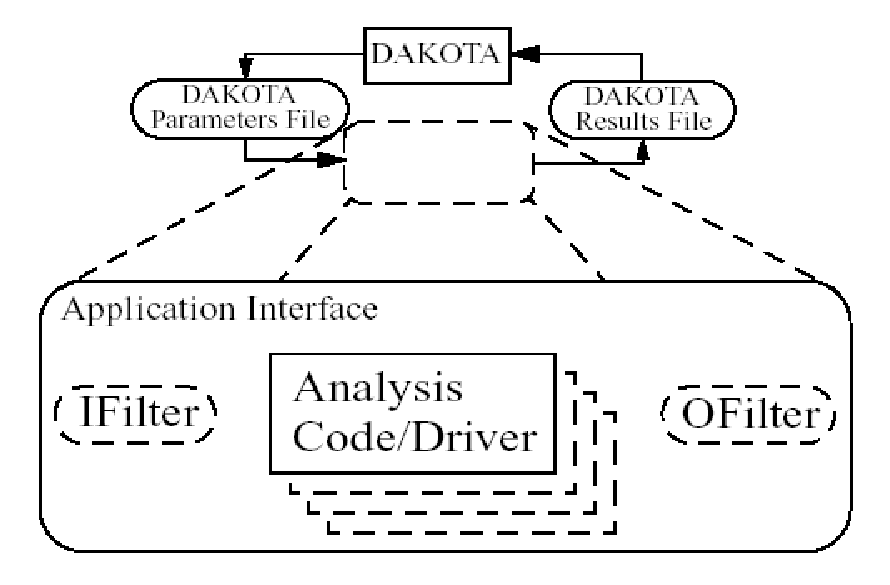
\includegraphics[scale=0.8]{images/dakota_components}
  \caption{Components of the simulation interface}
  \label{interfaces:bbinterfacecomp}
\end{figure}

When spawning function evaluations using system calls or forks, Dakota
must communicate parameter and response data with the analysis drivers
and filters through use of the file system. This is accomplished by
passing the names of the parameters and results files on the command
line when executing an analysis driver or filter. The input filter or
analysis driver read data from the parameters file and the output
filter or analysis driver write the appropriate data to the responses
file. While not essential when the file names are fixed, the file
names must be retrieved from the command line when Dakota is changing
the file names from one function evaluation to the next (i.e., using
temporary files or root names tagged with numerical identifiers).
In the case of a UNIX C-shell script, the two command line arguments
are retrieved using \texttt{\$argv[1]} and \texttt{\$argv[2]}
(see~\cite{And86}).  Similarly, Bourne shell scripts retrieve the two
command line arguments using \texttt{\$1} and \texttt{\$2}, and Perl
scripts retrieve the two command line arguments using
\texttt{@ARGV[0]} and \texttt{@ARGV[1]}.  In the case of a C or C++
program, command line arguments are retrieved using \texttt{argc}
(argument count) and \texttt{argv} (argument vector)~\cite{Ker88}, and
for Fortran 77, the \texttt{iargc} function returns the argument count
and the \texttt{getarg} subroutine returns command line arguments.

\subsection{Single analysis driver without filters}\label{interfaces:components:single1}

If a single \texttt{analysis\_driver} is selected in the interface
specification and filters are not needed (as indicated by omission of
the \texttt{input\_filter} and \texttt{output\_filter}
specifications), then only one process will appear in the execution
syntax of the simulation interface. An example of this syntax in the
system call case is:
\begin{small}
\begin{verbatim}
    driver params.in results.out
\end{verbatim}
\end{small}

where ``\path{driver}'' is the user-specified analysis driver and
``\path{params.in}'' and ``\path{results.out}'' are the names of the
parameters and results files, respectively, passed on the command
line. In this case, the user need not retrieve the command line
arguments since the same file names will be used each time.

For the same mapping, the fork simulation interface echoes the
following syntax:
\begin{small}
\begin{verbatim}
    blocking fork: driver params.in results.out
\end{verbatim}
\end{small}

for which only a single blocking fork is needed to perform the
evaluation.

Executing the same mapping with the direct simulation interface
results in an echo of the following syntax:
\begin{small}
\begin{verbatim}
    Direct function: invoking driver
\end{verbatim}
\end{small}

where this analysis driver must be linked as a function within
Dakota's direct interface (see Section~\ref{advint:direct}). Note that
no parameter or response files are involved, since such values
are passed directly through the function argument lists.

Both the system call and fork interfaces support asynchronous
operations. The asynchronous system call execution syntax involves
executing the system call in the background:
\begin{small}
\begin{verbatim}
    driver params.in.1 results.out.1 &
\end{verbatim}
\end{small}

and the asynchronous fork execution syntax involves use of a
nonblocking fork:
\begin{small}
\begin{verbatim}
    nonblocking fork: driver params.in.1 results.out.1
\end{verbatim}
\end{small}

where file tagging (see Section~\ref{interfaces:file:tagging1}) has
been user-specified in both cases to prevent conflicts between
concurrent analysis drivers. In these cases, the user must retrieve
the command line arguments since the file names change on each
evaluation.  Execution of the direct interface must currently be
performed synchronously since multithreading is not yet supported
(see Section~\ref{parallel:SLP:local:direct}).

\subsection{Single analysis driver with filters}\label{interfaces:components:single2}

When filters are used, the syntax of the system call that Dakota
performs is:
\begin{small}
\begin{verbatim}
    ifilter params.in results.out; driver params.in results.out;
         ofilter params.in results.out
\end{verbatim}
\end{small}

in which the input filter (``\path{ifilter}''), analysis driver
(``\path{driver}''), and output filter (``\path{ofilter}'')
processes are combined into a single system call through the use of
semi-colons (see~\cite{And86}). All three portions are
passed the names of the parameters and results files on the command
line.

For the same mapping, the fork simulation interface echoes the
following syntax:
\begin{small}
\begin{verbatim}
    blocking fork: ifilter params.in results.out;
         driver params.in results.out; ofilter params.in results.out
\end{verbatim}
\end{small}

where a series of three blocking forks is used to perform the
evaluation.

Executing the same mapping with the direct simulation interface
results in an echo of the following syntax:
\begin{small}
\begin{verbatim}
    Direct function: invoking { ifilter driver ofilter }
\end{verbatim}
\end{small}

where each of the three components must be linked as a function within
Dakota's direct interface. Since asynchronous operations are not yet
supported, execution simply involves invocation of each of the three
linked functions in succession. Again, no files are involved since
parameter and response data are passed directly through the function
argument lists.

Asynchronous executions would appear as follows for the system call
interface:
\begin{small}
\begin{verbatim}
    (ifilter params.in.1 results.out.1; driver params.in.1 results.out.1;
         ofilter params.in.1 results.out.1) &
\end{verbatim}
\end{small}

and, for the fork interface, as:
\begin{small}
\begin{verbatim}
    nonblocking fork: ifilter params.in.1 results.out.1;
         driver params.in.1 results.out.1; ofilter params.in.1 results.out.1
\end{verbatim}
\end{small}

where file tagging of evaluations has again been user-specified in
both cases. For the system call simulation interface, use of
parentheses and semi-colons to bind the three processes into a single
system call simplifies asynchronous process management compared to an
approach using separate system calls. The fork simulation interface,
on the other hand, does not rely on parentheses and accomplishes
asynchronous operations by first forking an intermediate process. This
intermediate process is then reforked for the execution of the input
filter, analysis driver, and output filter. The intermediate process
can be blocking or nonblocking (nonblocking in this case), and the
second level of forks can be blocking or nonblocking (blocking in this
case). The fact that forks can be reforked multiple times using either
blocking or nonblocking approaches provides the enhanced flexibility
to support a variety of local parallelism approaches (see
Chapter~\ref{parallel}).

\subsection{Multiple analysis drivers without filters}\label{interfaces:components:multiple1}

If a list of \texttt{analysis\_drivers} is specified and filters are
not needed (i.e., neither \texttt{input\_filter} nor
\texttt{output\_filter} appears), then the system call syntax
would appear as:
\begin{small}
\begin{verbatim}
    driver1 params.in results.out.1; driver2 params.in results.out.2;
         driver3 params.in results.out.3
\end{verbatim}
\end{small}

where ``\path{driver1}'', ``\path{driver2}'', and
``\path{driver3}'' are the user-specified analysis drivers and
``\path{params.in}'' and ``\path{results.out}'' are the
user-selected names of the parameters and results files. Note that the
results files for the different analysis drivers have been
automatically tagged to prevent overwriting. This automatic tagging of
\emph{analyses} (see Section~\ref{interfaces:file:tagging2}) is a
separate operation from user-selected tagging of \emph{evaluations}
(see Section~\ref{interfaces:file:tagging1}).

For the same mapping, the fork simulation interface echoes the
following syntax:
\begin{small}
\begin{verbatim}
    blocking fork: driver1 params.in results.out.1;
         driver2 params.in results.out.2; driver3 params.in results.out.3
\end{verbatim}
\end{small}

for which a series of three blocking forks is needed (no reforking of
an intermediate process is required).

Executing the same mapping with the direct simulation interface
results in an echo of the following syntax:
\begin{small}
\begin{verbatim}
    Direct function: invoking { driver1 driver2 driver3 }
\end{verbatim}
\end{small}

where, again, each of these components must be linked within Dakota's
direct interface and no files are involved for parameter and response
data transfer.

Both the system call and fork interfaces support asynchronous function
evaluations. The asynchronous system call execution syntax would be
reported as
\begin{small}
\begin{verbatim}
    (driver1 params.in.1 results.out.1.1; driver2 params.in.1 results.out.1.2;
         driver3 params.in.1 results.out.1.3) &
\end{verbatim}
\end{small}

and the nonblocking fork execution syntax would be reported as
\begin{small}
\begin{verbatim}
    nonblocking fork: driver1 params.in.1 results.out.1.1;
         driver2 params.in.1 results.out.1.2; driver3 params.in.1 results.out.1.3
\end{verbatim}
\end{small}

where, in both cases, file tagging of evaluations has been
user-specified to prevent conflicts between concurrent analysis
drivers and file tagging of the results files for multiple analyses is
automatically used. In the fork interface case, an intermediate
process is forked to allow a non-blocking function evaluation, and
this intermediate process is then reforked for the execution of each
of the analysis drivers.

\subsection{Multiple analysis drivers with filters}\label{interfaces:components:multiple2}

Finally, when combining filters with multiple
\texttt{analysis\_drivers}, the syntax of the system call that Dakota
performs is:
\begin{small}
\begin{verbatim}
    ifilter params.in.1 results.out.1;
         driver1 params.in.1 results.out.1.1;
         driver2 params.in.1 results.out.1.2;
         driver3 params.in.1 results.out.1.3;
         ofilter params.in.1 results.out.1
\end{verbatim}
\end{small}

in which all processes have again been combined into a single system
call through the use of semi-colons and parentheses. Note that the
secondary file tagging for the results files is only used for the
analysis drivers and not for the filters. This is consistent with the
filters' defined purpose of managing the non-repeated portions of
analysis pre- and post-processing (e.g., overlay of response results
from individual analyses; see Section~\ref{interfaces:file:tagging2}
for additional information).

For the same mapping, the fork simulation interface echoes the
following syntax:
\begin{small}
\begin{verbatim}
    blocking fork: ifilter params.in.1 results.out.1;
         driver1 params.in.1 results.out.1.1;
         driver2 params.in.1 results.out.1.2;
         driver3 params.in.1 results.out.1.3;
         ofilter params.in.1 results.out.1
\end{verbatim}
\end{small}

for which a series of five blocking forks is used (no reforking of an
intermediate process is required).

Executing the same mapping with the direct simulation interface
results in an echo of the following syntax:
\begin{small}
\begin{verbatim}
    Direct function: invoking { ifilter driver1 driver2 driver3 ofilter }
\end{verbatim}
\end{small}

where each of these components must be linked as a function within
Dakota's direct interface. Since asynchronous operations are not
supported, execution simply involves invocation of each of the five
linked functions in succession. Again, no files are involved for
parameter and response data transfer since this data is passed
directly through the function argument lists.

Asynchronous executions would appear as follows for the system call
interface:
\begin{small}
\begin{verbatim}
    (ifilter params.in.1 results.out.1;
         driver1 params.in.1 results.out.1.1;
         driver2 params.in.1 results.out.1.2;
         driver3 params.in.1 results.out.1.3;
         ofilter params.in.1 results.out.1) &
\end{verbatim}
\end{small}

and for the fork interface:
\begin{small}
\begin{verbatim}
    nonblocking fork: ifilter params.in.1 results.out.1;
         driver1 params.in.1 results.out.1.1;
         driver2 params.in.1 results.out.1.2;
         driver3 params.in.1 results.out.1.3;
         ofilter params.in.1 results.out.1
\end{verbatim}
\end{small}

where, again, user-selected file tagging of evaluations is combined
with automatic file tagging of analyses. In the fork interface case,
an intermediate process is forked to allow a non-blocking function
evaluation, and this intermediate process is then reforked for the
execution of the input filter, each of the analysis drivers, and the
output filter.

A complete example of these filters and multi-part drivers can be
found in \path{dakota/share/dakota/test/dakota_3pc/dakota_3pc.in}.

\section{Simulation File Management}\label{interfaces:file}

This section describes some management features used for files that
transfer data between Dakota and simulation codes
(i.e., when the system call or fork interfaces are used). These
features can generate unique filenames when
Dakota executes programs in parallel and can help one debug
the interface between Dakota and a simulation code.

\subsection{File Saving}\label{interfaces:file:saving}

{\bf Before driver execution:} In Dakota 5.0 and newer, an existing
results file will be removed immediately prior to executing the
analysis driver.  This new behavior addresses a common user problem
resulting from starting Dakota with stale results files in the run
directory.  To override this default behavior and preserve any
existing results files, specify \texttt{allow\_existing\_results}.

{\bf After driver execution:} The \texttt{file\_save} option in the
interface specification allows the user to control whether parameters
and results files are retained or removed from the working directory
after the analysis completes. Dakota's default behavior is to remove
files once their use is complete to reduce clutter. If the method
output setting is verbose, a file remove notification will follow the
function evaluation echo, e.g.,
\begin{small}
\begin{verbatim}
    driver /usr/tmp/aaaa20305 /usr/tmp/baaa20305
    Removing /usr/tmp/aaaa20305 and /usr/tmp/baaa20305
\end{verbatim}
\end{small}

However, if \texttt{file\_save} appears in the interface
specification, these files will not be removed. This latter behavior
is often useful for debugging communication between Dakota and
simulator programs. An example of a \texttt{file\_save} specification
is shown in the file tagging example below.

\subsection{File Tagging for Evaluations}\label{interfaces:file:tagging1}

When a user provides \texttt{parameters\_file} and
\texttt{results\_file} specifications, the \texttt{file\_tag} option
in the interface specification causes Dakota to make the names of
these files unique by appending the function
evaluation number to the root file names. Default behavior is to not
tag these files, which has the advantage of allowing the user to
ignore command line argument passing and always read to and write from
the same file names. However, it has the disadvantage that files may
be overwritten from one function evaluation to the next. When
\texttt{file\_tag} appears in the interface specification, the file names
are made unique by the appended evaluation number. This uniqueness
requires the user's interface to get the names of
these files from the command line. The file tagging feature is most
often used when concurrent simulations are running in a common disk
space, since it can prevent conflicts between the simulations. An
example specification of \texttt{file\_tag} and \texttt{file\_save} is
shown below:
\begin{small}
\begin{verbatim}
    interface,
            system
              analysis_driver = 'text_book'
              parameters_file = 'text_book.in'
              results_file    = 'text_book.out'
              file_tag file_save
\end{verbatim}
\end{small}

\emph{Special case:} When a user specifies names for the parameters
and results files and \texttt{file\_save} is used without
\texttt{file\_tag}, untagged files are used in the function evaluation
but are then moved to tagged files after the function evaluation is
complete, to prevent overwriting files for which a
\texttt{file\_save} request has been given. If the output control is
set to verbose, then a notification similar to the following will
follow the function evaluation echo:
\begin{small}
\begin{verbatim}
    driver params.in results.out
    Files with non-unique names will be tagged to enable file_save:
    Moving params.in to params.in.1
    Moving results.out to results.out.1
\end{verbatim}
\end{small}

\textbf{Hierarchical tagging:} When a model's specification includes
the {\tt hierarchical\_tagging} keyword, the tag applied to parameter
and results file names of any subordinate interfaces will reflect any
model hierarchy present.  This option is useful for studies involving
multiple models with a nested or hierarchical relationship.  For
example a nested model has a sub-method, which itself likely operates
on a sub-model, or a hierarchical approximation involves coordination
of low and high fidelity models.  Specifying {\tt
hierarchical\_tagging} will yield function evaluation identifiers
(``tags'') composed of the evaluation IDs of the models involved,
e.g., outermodel.innermodel.interfaceid = 4.9.2.  This communicates
the outer contexts to the analysis driver when performing a function
evaluation.  For an example of using hierarchical tagging in a nested
model context,
see \path{dakota/share/dakota/test/dakota_uq_timeseries_*_optinterf.in}.

\subsection{Temporary Files}\label{interfaces:file:temporary}

If \texttt{parameters\_file} and \texttt{results\_file} are not
specified by the user, temporary files having generated names are
used.  For example, a system call to a single analysis driver might
appear as:
\begin{small}
\begin{verbatim}
    driver /tmp/dakota_params_aaaa2035 /tmp/dakota_results_baaa2030
\end{verbatim}
\end{small}

and a system call to an analysis driver with filter programs might appear as:
\begin{small}
\begin{verbatim}
    ifilter /tmp/dakota_params_aaaa2490 /tmp/dakota_results_baaa2490;
         driver /tmp/dakota_params_aaaa2490 tmp/dakota_results_baaa2490;
         ofilter /tmp/dakota_params_aaaa2490 /tmp/dakota_results_baa22490
\end{verbatim}
\end{small}

These files have unique names created by Boost filesystem
utilities. This uniqueness requires the user's interface to get the
names of these files from the command line. File tagging with
evaluation number is unnecessary with temporary files, but can be
helpful for the user workflow to identify the evaluation number.  Thus
\texttt{file\_tag} requests will be honored. A \texttt{file\_save}
request will be honored, but it should be used with care since the
temporary file directory could easily become cluttered without the
user noticing.

\subsection{File Tagging for Analysis Drivers}\label{interfaces:file:tagging2}

When multiple analysis drivers are involved in performing a function
evaluation with either the system call or fork simulation interface,
a secondary file tagging is \emph{automatically} used to
distinguish the results files used for the individual analyses. This
applies to both the case of user-specified names for the parameters
and results files and the default temporary file case. Examples
for the former case were shown previously in
Section~\ref{interfaces:components:multiple1} and
Section~\ref{interfaces:components:multiple2}.  The following examples
demonstrate the latter temporary file case. Even though Unix
temporary files have unique names for a particular function
evaluation, tagging is still needed to manage the individual
contributions of the different analysis drivers to the response
results, since the same root results filename is used for each
component. For the system call interface, the syntax would be similar
to the following:
\begin{small}
\begin{verbatim}
    ifilter /var/tmp/aaawkaOKZ /var/tmp/baaxkaOKZ;
         driver1 /var/tmp/aaawkaOKZ /var/tmp/baaxkaOKZ.1;
         driver2 /var/tmp/aaawkaOKZ /var/tmp/baaxkaOKZ.2;
         driver3 /var/tmp/aaawkaOKZ /var/tmp/baaxkaOKZ.3;
         ofilter /var/tmp/aaawkaOKZ /var/tmp/baaxkaOKZ
\end{verbatim}
\end{small}

and, for the fork interface, similar to:
\begin{small}
\begin{verbatim}
    blocking fork:
         ifilter /var/tmp/aaawkaOKZ /var/tmp/baaxkaOKZ;
         driver1 /var/tmp/aaawkaOKZ /var/tmp/baaxkaOKZ.1;
         driver2 /var/tmp/aaawkaOKZ /var/tmp/baaxkaOKZ.2;
         driver3 /var/tmp/aaawkaOKZ /var/tmp/baaxkaOKZ.3;
         ofilter /var/tmp/aaawkaOKZ /var/tmp/baaxkaOKZ
\end{verbatim}
\end{small}

Tagging of results files with an analysis identifier is needed
since each analysis driver must contribute a
user-defined subset of the total response results for the evaluation.
If an output filter is not supplied, Dakota will combine these
portions through a simple overlaying of the individual contributions
(i.e., summing the results in \path{/var/tmp/baaxkaOKZ.1},
\path{/var/tmp/baaxkaOKZ.2}, and \path{/var/tmp/baaxkaOKZ.3}). If
this simple approach is inadequate, then an output filter should be
supplied to perform the combination. This is the reason why the
results file for the output filter does not use analysis tagging; it
is responsible for the results combination (i.e., combining
\path{/var/tmp/baaxkaOKZ.1}, \path{/var/tmp/baaxkaOKZ.2}, and
\path{/var/tmp/baaxkaOKZ.3} into \path{/var/tmp/baaxkaOKZ}). In
this case, Dakota will read only the results file from the output
filter (i.e., \path{/var/tmp/baaxkaOKZ}) and interpret it as the
total response set for the evaluation.

Parameters files are not currently tagged with an analysis identifier.
This reflects the fact that Dakota does not attempt to subdivide the
requests in the active set vector for different analysis portions.
Rather, the total active set vector is passed to each analysis driver
and the appropriate subdivision of work \emph{must be defined by the
  user}. This allows the division of labor to be very flexible. In
some cases, this division might occur across response functions, with
different analysis drivers managing the data requests for different
response functions. And in other cases, the subdivision might occur
within response functions, with different analysis drivers
contributing portions to each of the response functions. The only
restriction is that each of the analysis drivers must follow the
response format dictated by the total active set vector. For response
data for which an analysis driver has no contribution, 0's must be
used as placeholders.

\subsection{Work Directories}\label{interfaces:workdir}

Sometimes it is convenient for simulators and filters to run in a
directory different from the one where Dakota is invoked.  For instance,
when performing concurrent evaluations and/or analyses, it is often
necessary to cloister input and output files in separate directories to
avoid conflicts.  A simulator script used as an \texttt{analysis\_driver}
can of course include commands to change to a different directory if
desired (while still arranging to write a results file in the original
directory), but Dakota has facilities that may simplify the creation of
simulator scripts.  When the \texttt{work\_directory} feature is enabled,
Dakota will create a directory for each evaluation/analysis (with
optional tagging and saving as with files).  To enable the
\texttt{work\_directory} feature an interface specification includes
the keyword
\begin{small}
\begin{verbatim}
       work_directory
\end{verbatim}
\end{small}
then Dakota will arrange for the simulator and any filters to
wake up in the work directory, with \$PATH adjusted (if necessary)
so programs that could be invoked without a relative
path to them (i.e., by a name not involving any slashes) from
Dakota's directory can also be invoked from the simulator's (and filter's)
directory.  On occasion, it is convenient for the simulator to have
various files, e.g., data files, available in the directory where it
runs.  If, say, \path{my/special/directory/} is such a directory
(as seen from Dakota's directory), the interface specification
\begin{small}
\begin{verbatim}
       work_directory named 'my/special/directory'
\end{verbatim}
\end{small}
would cause Dakota to start the simulator and any filters in that
directory.  If the directory did not already exist, Dakota would
create it and would remove it after the simulator (or output filter,
if specified) finished, unless instructed not to do so by the
appearance of \texttt{directory\_save} (or its deprecated synonym
\texttt{dir\_save}) in the interface specification.  If \texttt{named
  '$...$'} does not appear, then \texttt{directory\_save} cannot
appear either, and Dakota creates a temporary directory (using the
\texttt{tmpnam} function to determine its name) for use by the
simulator and any filters.  If you specify \texttt{directory\_tag} (or
the deprecated \texttt{dir\_tag}), Dakota causes each invocation of
the simulator and any filters to start in a subdirectory of the work
directory with a name composed of the work directory's name followed
by a period and the invocation number (1, 2, $...$); this might be
useful in debugging.

Sometimes it can be helpful for the simulator and filters to start in a
new directory populated with some files.  Adding
\begin{small}
\begin{verbatim}
       link_files 'templatedir/*'
\end{verbatim}
\end{small}
to the work directory specification would cause the
contents of directory \path{templatedir/} to be linked
into the work directory.  Linking makes sense if files are large,
but when practical, it is far more reliable to have
copies of the files; adding \texttt{copy\_files} to the specification
would cause the contents of the template directory to be copied
to the work directory.  The linking or copying does
not overwrite existing files unless \texttt{replace} also appears
in the specification.

Here is a summary of possibilities for a work directory specification,
with {\tt\verb=[=$...$\verb=]=} denoting that $...$ is optional:
\begin{small}
\begin{verbatim}
  work_directory [ named '...' ]
    [ directory_tag ]     # (or dir_tag)
    [ directory_save ]    # (or dir_save)
    [ link_files '...' '...' ]
    [ copy_files '...' '...' ]
    [ replace ]
\end{verbatim}
\end{small}

Figure~\ref{fig:interface:workdir} contains an example of these
specifications in a Dakota input file for constrained optimization.
\begin{figure}
  \centering
  \begin{bigbox}
    \begin{small}
      \verbatimtabinput[8]{../../test/examples-users/workdir_textbook.in}
    \end{small}
  \end{bigbox}
  \caption{The \protect\path{workdir_textbook.in} input file.}
  \label{fig:interface:workdir}
\end{figure}

\section{Batched Evaluations}\label{interfaces:batch}

Beginning with release 6.11, Dakota provides for execution of
evaluations in batches. Batch mode is intended to allow a user
to assume greater control over where and when to run individual
evaluations. It is activated using the \texttt{batch} keyword.

In batch mode, Dakota writes the parameters for multiple (a batch of)
evaluations to a single batch parameters file and then invokes the
analysis driver once for the entire batch. The pathname of the
combined parameters file (and of the results file) are communicated
to the driver as command line arguments. After the driver exits, Dakota
expects to find results for the entire batch in a single combined results
file.

The analysis driver is responsible for parsing the parameters file
and performing an evaluation for each set of parameters it contains,
and for returning results for all the evaluations to Dakota. The user
is free to set up the driver to perform the evaluations in the batch in
a way that is convenient.

By default, all currently available evaluations are added to a single
batch. For example, in a sampling study that has a 1000 samples, by
default all 1000 evaluations would be added to a single batch. The batch
size may be limited using the \texttt{size} subkeyword. Setting 
\texttt{size = 100} would result in 10 equal-size batches being run one
after another in a 1000-sample study. 

\subsection{File Formats}

The combined parameters file for a batch is simply the concatenation of 
all the parameters files for the evaluations in the batch. The individual
parameter sets may use the default Dakota format, or the user can select
the aprepro format.

The following example parameters file contains parameter sets for two
evaluations. 

\begin{small}
\begin{verbatim}
                                          1 variables
                     -4.912558193411678e-01 x1
                                          1 functions
                                          1 ASV_1:response_fn_1
                                          1 derivative_variables
                                          1 DVV_1:x1
                                          0 analysis_components
                                        1:1 eval_id
                                          1 variables
                     -2.400695372000337e-01 x1
                                          1 functions
                                          1 ASV_1:response_fn_1
                                          1 derivative_variables
                                          1 DVV_1:x1
                                          0 analysis_components
                                        1:2 eval_id    interface,
\end{verbatim}
\end{small}

Note that the \texttt{eval\_id} contains two pieces of 
information separated by a colon. The second is the evaluation number,
and the first is the batch number. The batch number is an incrementing
integer that uniquely identifies the batch.

The combined results file format is likewise a concatenation of the results
for all the evaluations in the batch. However, a line beginning with the
``\#'' character must separate the results for each evaluation.

The order of the evaluations in the results file must match the order in the
parameters file.

The following is an example batch results file corresponding to the batch
parameters file above. The initial \# on the first line is optional, and a
final \# (not shown here) is allowed.
\begin{small}
\begin{verbatim}
#
                     4.945481774823024e+00 f
#
                     2.364744129789246e+00 f
\end{verbatim}
\end{small}


\subsection{Work Directories, Tagging, and Other Features}

Each batch is executed in a work directory when this feature is enabled.
The batch number is used to tag files and directories if tagging is requested
(or Dakota automatically applies a tag to safely save a file or directory). As
explained in the previous section, the batch number is an incrementing integer
beginning with 1 that uniquely identifies a batch.

Batch mode restricts the use of several other Dakota features.

\begin{itemize}

  \item No \texttt{input\_filter} or \texttt{output\_filter} is allowed.
  \item Only one \texttt{analysis\_driver} is permitted.
  \item \texttt{failure\_capture} modes are limited to abort and recover.
  \item Asynchronous evaluation is disallowed (only one batch at a time may be executed).
\end{itemize}


\section{Parameter to Response Mapping Examples}\label{interfaces:mappings}

In this section, interface mapping examples are presented through the
discussion of several parameters files and their corresponding results
files. A typical input file for 2 variables ($n=2$) and 3 functions
($m=3$) using the standard parameters file format (see
Section~\ref{variables:parameters:standard}) is as follows:
\begin{small}
\begin{verbatim}
                        2 variables
    1.500000000000000e+00 cdv_1
    1.500000000000000e+00 cdv_2
                        3 functions
                        1 ASV_1
                        1 ASV_2
                        1 ASV_3
                        2 derivative_variables
                        1 DVV_1
                        2 DVV_2
                        0 analysis_components
\end{verbatim}
\end{small}
where numerical values are associated with their tags within
``\texttt{value tag}'' constructs. The number of design variables
($n$) and the string ``\texttt{variables}'' are followed by the values
of the design variables and their tags, the number of functions ($m$)
and the string ``\texttt{functions}'', the active set vector (ASV) and
its tags, the number of derivative variables and the string
``\texttt{derivative\_variables}'', the derivative variables vector
(DVV) and its tags, the number of analysis components and the string
``\texttt{analysis\_components}'', and the analysis components array
and its tags.  The descriptive tags for the variables are always
present and they are either the descriptors in the user's variables
specification, if given there, or are default descriptors.  The length
of the active set vector is equal to the number
of functions ($m$). In the case of an optimization data set with an
objective function and two nonlinear constraints (three response
functions total), the first ASV value is associated with the objective
function and the remaining two are associated with the constraints (in
whatever consistent constraint order has been defined by the user).
The DVV defines a subset of the variables used for computing
derivatives.  Its identifiers are 1-based and correspond to the full
set of variables listed in the first array.  Finally, the analysis
components pass additional strings from the user's
\texttt{analysis\_components} specification in a Dakota input file
through to the simulator.  They allow the development of simulation
drivers that are more flexible, by allowing them to be passed
additional specifics at run time, e.g., the names of model files such
as a particular mesh to use.

For the APREPRO format option (see
Section~\ref{variables:parameters:aprepro}), the same set of data
appears as follows:
\begin{small}
\begin{verbatim}
    { DAKOTA_VARS     =                      2 }
    { cdv_1           =  1.500000000000000e+00 }
    { cdv_2           =  1.500000000000000e+00 }
    { DAKOTA_FNS      =                      3 }
    { ASV_1           =                      1 }
    { ASV_2           =                      1 }
    { ASV_3           =                      1 }
    { DAKOTA_DER_VARS =                      2 }
    { DVV_1           =                      1 }
    { DVV_2           =                      2 }
    { DAKOTA_AN_COMPS =                      0 }
\end{verbatim}
\end{small}

where the numerical values are associated with their tags within
``\texttt{\{ tag = value \}}'' constructs.

The user-supplied simulation interface, comprised of a simulator
program or driver and (optionally) filter programs, is responsible for
reading the parameters file and creating a results file that contains
the response data requested in the ASV. This response data is written
in the format described in Section~\ref{responses:results}. Since the
ASV contains all ones in this case, the response file corresponding to
the above input file would contain values for the three functions:
\begin{small}
\begin{verbatim}
    1.250000000000000e-01 f
    1.500000000000000e+00 c1
    1.500000000000000e+00 c2
\end{verbatim}
\end{small}

Since function tags are optional, the following would be equally
acceptable:
\begin{small}
\begin{verbatim}
    1.250000000000000e-01
    1.500000000000000e+00
    1.500000000000000e+00
\end{verbatim}
\end{small}

For the same parameters with different ASV components,
\begin{small}
\begin{verbatim}
                        2 variables
    1.500000000000000e+00 cdv_1
    1.500000000000000e+00 cdv_2
                        3 functions
                        3 ASV_1
                        3 ASV_2
                        3 ASV_3
                        2 derivative_variables
                        1 DVV_1
                        2 DVV_2
                        0 analysis_components
\end{verbatim}
\end{small}

the following response data is required:
\begin{small}
\begin{verbatim}
    1.250000000000000e-01 f
    1.500000000000000e+00 c1
    1.500000000000000e+00 c2
    [ 5.000000000000000e-01 5.000000000000000e-01 ]
    [ 3.000000000000000e+00 -5.000000000000000e-01 ]
    [ -5.000000000000000e-01 3.000000000000000e+00 ]
\end{verbatim}
\end{small}
Here, we need not only the function values, but also each of their
gradients. The derivatives are computed with respect to \texttt{cdv\_1}
and \texttt{cdv\_2} as indicated by the DVV values. Another modification
to the ASV components yields the following parameters file:
\begin{small}
\begin{verbatim}
                        2 variables
    1.500000000000000e+00 cdv_1
    1.500000000000000e+00 cdv_2
                        3 functions
                        2 ASV_1
                        0 ASV_2
                        2 ASV_3
                        2 derivative_variables
                        1 DVV_1
                        2 DVV_2
                        0 analysis_components
\end{verbatim}
\end{small}

for which the following results file is needed:
\begin{small}
\begin{verbatim}
    [ 5.000000000000000e-01 5.000000000000000e-01 ]
    [ -5.000000000000000e-01 3.000000000000000e+00 ]
\end{verbatim}
\end{small}
Here, we need gradients for functions \texttt{f} and \texttt{c2}, but
not for \texttt{c1}, presumably since this constraint is inactive.

A full Newton optimizer might make the following request:
\begin{small}
\begin{verbatim}
                        2 variables
    1.500000000000000e+00 cdv_1
    1.500000000000000e+00 cdv_2
                        1 functions
                        7 ASV_1
                        2 derivative_variables
                        1 DVV_1
                        2 DVV_2
                        0 analysis_components
\end{verbatim}
\end{small}

for which the following results file,
\begin{small}
\begin{verbatim}
    1.250000000000000e-01 f
    [ 5.000000000000000e-01 5.000000000000000e-01 ]
    [[ 3.000000000000000e+00 0.000000000000000e+00
       0.000000000000000e+00 3.000000000000000e+00 ]]
\end{verbatim}
\end{small}
containing the objective function, its gradient vector, and its
Hessian matrix, is needed.  Again, the derivatives (gradient vector
and Hessian matrix) are computed with respect to \texttt{cdv\_1} and
\texttt{cdv\_2} as indicated by the DVV values.

Lastly, a more advanced example could have multiple types of variables
present; in this example, 2 continuous design and 3 discrete design
range, 2 normal uncertain, and 3 continuous state and 2 discrete state
range variables.  When a mixture of variable types is present, the
content of the DVV (and therefore the required length of gradient
vectors and Hessian matrices) depends upon the type of study being
performed (see Section~\ref{responses:active}).  For a reliability
analysis problem, the uncertain variables are the active continuous
variables and the following parameters file would be typical:
\begin{small}
\begin{verbatim}
                       12 variables
    1.500000000000000e+00 cdv_1
    1.500000000000000e+00 cdv_2
                        2 ddriv_1
                        2 ddriv_2
                        2 ddriv_3
    5.000000000000000e+00 nuv_1
    5.000000000000000e+00 nuv_2
    3.500000000000000e+00 csv_1
    3.500000000000000e+00 csv_2
    3.500000000000000e+00 csv_3
                        4 dsriv_1
                        4 dsriv_2
                        3 functions
                        3 ASV_1
                        3 ASV_2
                        3 ASV_3
                        2 derivative_variables
                        6 DVV_1
                        7 DVV_2
                        2 analysis_components
                mesh1.exo AC_1
                  db1.xml AC_2
\end{verbatim}
\end{small}

Gradients are requested with respect to variable entries 6 and 7,
which correspond to normal uncertain variables \texttt{nuv\_1} and
\texttt{nuv\_2}.  The following response data would be appropriate:
\begin{small}
\begin{verbatim}
    7.943125000000000e+02 f
    1.500000000000000e+00 c1
    1.500000000000000e+00 c2
    [ 2.560000000000000e+02 2.560000000000000e+02 ]
    [ 0.000000000000000e+00 0.000000000000000e+00 ]
    [ 0.000000000000000e+00 0.000000000000000e+00 ]
\end{verbatim}
\end{small}

In a parameter study, however, no distinction is drawn between
different types of continuous variables, and derivatives would be
needed with respect to all continuous variables ($n_{dvv}=7$ for the
continuous design variables \texttt{cdv\_1} and \texttt{cdv\_2}, the
normal uncertain variables \texttt{nuv\_1} and \texttt{nuv\_2}, and
the continuous state variables \texttt{csv\_1}, \texttt{csv\_2} and
\texttt{csv\_3}).  The parameters file would appear as
\begin{small}
\begin{verbatim}
                       12 variables
    1.500000000000000e+00 cdv_1
    1.500000000000000e+00 cdv_2
                        2 ddriv_1
                        2 ddriv_2
                        2 ddriv_3
    5.000000000000000e+00 nuv_1
    5.000000000000000e+00 nuv_2
    3.500000000000000e+00 csv_1
    3.500000000000000e+00 csv_2
    3.500000000000000e+00 csv_3
                        4 dsriv_1
                        4 dsriv_2
                        3 functions
                        3 ASV_1
                        3 ASV_2
                        3 ASV_3
                        7 derivative_variables
                        1 DVV_1
                        2 DVV_2
                        6 DVV_3
                        7 DVV_4
                        8 DVV_5
                        9 DVV_6
                       10 DVV_7
                        2 analysis_components
                mesh1.exo AC_1
                  db1.xml AC_2
\end{verbatim}
\end{small}

and the corresponding results would appear as
\begin{small}
\begin{verbatim}
    7.943125000000000e+02 f
    1.500000000000000e+00 c1
    1.500000000000000e+00 c2
    [  5.000000000000000e-01  5.000000000000000e-01  2.560000000000000e+02
       2.560000000000000e+02  6.250000000000000e+01  6.250000000000000e+01
       6.250000000000000e+01 ]
    [  3.000000000000000e+00 -5.000000000000000e-01  0.000000000000000e+00
       0.000000000000000e+00  0.000000000000000e+00  0.000000000000000e+00
       0.000000000000000e+00 ]
    [ -5.000000000000000e-01  3.000000000000000e+00  0.000000000000000e+00
       0.000000000000000e+00  0.000000000000000e+00  0.000000000000000e+00
       0.000000000000000e+00 ]
\end{verbatim}
\end{small}

\section{Parameters and Results Files with dakota.interfacing}\label{interfaces:dakota.interfacing}

The Python module {\tt dakota.interfacing} first was made available with Dakota 6.6. (It was released with 
Dakota 6.5 as the module {\tt dipy}.) By providing a Python interface to read and write, respectively,
Dakota parameters and results files, {\tt dakota.interfacing} can simplify development of black-box
interfaces. The benefit may be greatest when one or more phases of the interface (pre-processing, execution,
post-processing) is written in Python.

The following sections describe the components of {\tt dakota.interfacing}. These components include:
\begin{itemize}
  \item The {\tt Parameters} class. Makes available the variable information for a single evaluation
  \item The {\tt Results} class. Collects results for a single evaluation and writes them to file 
  \item The {\tt BatchParameters} and {\tt BatchResults} classes. Containers for multiple {\tt Parameters} and 
	  {\tt Results} objects; used when evaluations are performed by Dakota in batch mode (Section~\ref{interfaces:batch})
  \item The {\tt read\_parameters\_file} function. Constructs {\tt Parameters}, 
        {\tt Results}, {\tt BatchParameters}, and {\tt BatchResults} objects from a Dakota 
        parameters file.
\end{itemize}

\subsection{Creating Parameters and Results objects}

{\tt dakota.interfacing} has one free function, {\tt read\_parameters\_file}, which creates {\tt Parameters}, 
{\tt Results}, {\tt BatchParameters}, and {\tt BatchResults} objects from a Dakota parameters file. For
single, non-batch evaluation, it returns a tuple that contains {\tt (Parameters, Results)}. For batch evaluations,
it instead returns a tuple containing {\tt (BatchParameters, BatchResults)}.

Its signature is:

\phantomsection\label{index:dakota.interfacing.read_parameters_file}\texttt{dakota.interfacing.}\textbf{\texttt{read\_parameters\_file}}({\emph{parameters\_file=None}, \emph{results\_file=None},\\\emph{ignore\_asv=False}, \emph{batch=False}}){}

\emph{parameters\_file} and \emph{results\_file} are the names of the parameters file that is to be read
and the results file that  ultimately is to be written. The names can be  absolute or relative filepaths or
just filenames. If a parameters file or results file is not provided, it will be obtained from the command 
line arguments. (The results filename is assumed to be the last command line argument, and the parameters 
file the second to last.) Note that if the working directory has changed since script invocation, filenames
provided as command line arguments by Dakota's {\tt fork} or {\tt system} interfaces may be incorrect.

If \emph{results\_file} is set to the constant {\tt dakota.interfacing.UNNAMED}, the {\tt Results} or 
{\tt BatchResults} object is constructed without a results file name.  In this case, an output stream must be 
provided when\\{\tt Results.write()} or {\tt BatchResults.write()} is called. Unnamed results files are most 
helpful when no results file will be written, as with a script intended purely for pre-processing.

By default, the returned {\tt Results} or {\tt BatchResults} object enforces the active set vector (see the 
{\tt Results} class section). This behavior can be overridden, allowing any property (function, gradient, Hessian) of 
a response to be set, by setting \emph{ignore\_asv} to {\tt True}. The \emph{ignore\_asv} option can be useful
when setting up or debugging a driver.

The {\tt batch} argument must be set to {\tt True} when batch evaluation has been requested in the Dakota input
file, and {\tt False} when not.

\subsection{Parameters objects}

{\tt Parameters} objects make the variables, analysis components, evaluation ID, and evaluation number read from a Dakota parameters file available through a combination of key-value access and object attributes. Although {\tt Parameters} objects may be constructed directly, it is advisable to use the {\tt read\_parameters\_file} function instead.

Variable values can be accessed by Dakota descriptor or by index using {[}{]} on the object itself. Variables types (integer, real, string) are inferred by first attempting to convert to {\tt int} and then, if this fails, to {\tt float}.

Analysis components are accessible by index only using the {\tt an\_comps} attribute. Iterating over a {\tt Parameters} 
object yields the variable descriptors.

{\tt Parameters} objects have the attributes:

\begin{itemize}

  \item\index{an\_comps (dakota.interfacing.Parameters attribute)} \phantomsection\label{index:dakota.interfacing.Parameters.an_comps}\textbf{\texttt{an\_comps}} List of the analysis components (strings).

  \item\index{eval\_id (dakota.interfacing.Parameters attribute)} \phantomsection\label{index:dakota.interfacing.Parameters.eval_id}\textbf{\texttt{eval\_id}} Evaluation id (string).

  \item\index{eval\_num (dakota.interfacing.Parameters attribute)} \phantomsection\label{index:dakota.interfacing.Parameters.eval_num}\textbf{\texttt{eval\_num}} Evaluation number (final token in eval\_id) (int).


  \item\index{aprepro\_format (dakota.interfacing.Parameters attribute)} \phantomsection\label{index:dakota.interfacing.Parameters.aprepro_format}\textbf{\texttt{aprepro\_format}} Boolean indicating whether the parameters file was in aprepro (True) or Dakota (False) format.

  \item\index{descriptors (dakota.interfacing.Parameters attribute)}\phantomsection\label{index:dakota.interfacing.Parameters.descriptors}\textbf{\texttt{descriptors}} List of the variable descriptors

  \item\index{num\_variables (dakota.interfacing.Parameters attribute)} \phantomsection\label{index:dakota.interfacing.Parameters.num_variables}\textbf{\texttt{num\_variables}} Number of variables

  \item\index{num\_an\_comps (dakota.interfacing.Parameters attribute)}\phantomsection\label{index:dakota.interfacing.Parameters.num_an_comps}\textbf{\texttt{num\_an\_comps}} Number of analysis components

\end{itemize}

Parameters objects have the methods:

\begin{itemize}
  \item\index{items() (dakota.interfacing.Parameters method)}
	  \phantomsection\label{index:dakota.interfacing.Parameters.items}\textbf{\texttt{items}}{()}{}
          Return an iterator that yields tuples of the descriptor and value for each parameter. ({\tt Results} objects also have {\tt items()}.)

  \item\index{values() (dakota.interfacing.Parameters method)}
	  \phantomsection\label{index:dakota.interfacing.Parameters.values}\textbf{\texttt{values}}{()}{}
          Return an iterator that yields the value for each parameter. ({\tt Results} objects have the corresponding method {\tt responses()}.)

\end{itemize}

\subsection{Results objects}

{\tt Results} objects:
\begin{itemize}

  \item communicate response requests from Dakota (active set vector and derivative variables)
  \item collect response data (function values, gradients, and Hessians)
  \item write Dakota results files
\end{itemize}

{\tt Results} objects are collections of {\tt Response} objects, which are documented in the following section. Each {\tt Response} can be accessed by name (Dakota descriptor) or by index using {[}{]} on the {\tt Results} object itself. Iterating over a {\tt Results} object yields the response descriptors. Although {\tt Results} objects may be constructed directly, it is advisable to use the {\tt read\_parameters\_file} function instead.

Results objects have the attributes:

\begin{itemize}

  \item\index{eval\_id (dakota.interfacing.Results attribute)} \phantomsection\label{index:dakota.interfacing.Results.eval_id}\textbf{\texttt{eval\_id}} Evaluation id (a string).

  \item\index{eval\_num (dakota.interfacing.Results attribute)} \phantomsection\label{index:dakota.interfacing.Results.eval_num}\textbf{\texttt{eval\_num}} Evaluation number (final token in eval\_id) (int).

  \item\index{aprepro\_format (dakota.interfacing.Results attribute)} \phantomsection\label{index:dakota.interfacing.Results.aprepro_format}\textbf{\texttt{aprepro\_format}} Boolean indicating whether the parameters file was in
aprepro (True) or Dakota (False) format.

  \item\index{descriptors (dakota.interfacing.Results attribute)} \phantomsection\label{index:dakota.interfacing.Results.descriptors}\textbf{\texttt{descriptors}} List of the response descriptors (strings)

  \item\index{num\_responses (dakota.interfacing.Results attribute)}  \phantomsection\label{index:dakota.interfacing.Results.num_responses}\textbf{\texttt{num\_responses}} Number of variables (read-only)

  \item\index{deriv\_vars (dakota.interfacing.Results attribute)} \phantomsection\label{index:dakota.interfacing.Results.deriv_vars}\textbf{\texttt{deriv\_vars}} List of the derivative variables (strings)

  \item\index{num\_deriv\_vars (dakota.interfacing.Results attribute)}\phantomsection\label{index:dakota.interfacing.Results.num_deriv_vars}\textbf{\texttt{num\_deriv\_vars}}Number of derivative variables (int)

\end{itemize}

Results objects have the methods:

\begin{itemize}
  \item\index{items() (dakota.interfacing.Results method)}
	  \phantomsection\label{index:dakota.interfacing.Results.items}\textbf{\texttt{items}}{()}{}
          Return an iterator that yields tuples of the descriptor and {\tt Response} object for each response. ({\tt Parameters} objects also have {\tt items()}.)

  \item\index{responses() (dakota.interfacing.Results method)}
	  \phantomsection\label{index:dakota.interfacing.Results.responses}\textbf{\texttt{responses}}{()}{}
          Return an iterator that yields the {\tt Response} object for each response. ({\tt Parameters} objects have the corresponding method {\tt values()}.)

  \item\index{fail() (dakota.interfacing.Results method)}
	  \phantomsection\label{index:dakota.interfacing.Results.fail}\textbf{\texttt{fail}}{()}{}
	  Set the FAIL attribute. When the results file is written, it will contain only the word FAIL, triggering Dakota's failure capturing behavior (See Chapter~\ref{failure}).

\item \index{write() (dakota.interfacing.Results method)}
	\phantomsection\label{index:dakota.interfacing.Results.write}\textbf{\texttt{write}}({\emph{stream=None}, \emph{ignore\_asv=None}}){}
Write the results to the Dakota results file. If \emph{stream} is set, it overrides the results file name provided at construct time. It must be an open file-like object, rather than the name of a file. If \emph{ignore\_asv} is True, the file will be written even if information requested via the active set vector is missing. Calling {\tt write()} on a {\tt Results} object that was
generated by reading a batch parameters file will raise a {\tt BatchWriteError}. Instead, {\tt write()} should be called on
the containing {\tt BatchResults} object.

\end{itemize}

\subsection{Response object}

{\tt Response} objects store response information. They typically are instantiated and accessed through a Results object by index or response descriptor using {[}{]}.

{\tt Response}s have the attributes:

\begin{itemize}
  \item \index{asv (dakota.interfacing.Response attribute)} \phantomsection\label{index:dakota.interfacing.Response.asv}\textbf{\texttt{asv}} a {\tt collections.namedtuple} with three members, \emph{function}, \emph{gradient}, and \emph{hessian}.
Each is a boolean indicating whether Dakota requested the
associated information for the response. {\tt namedtuples} can be
accessed by index or by member.

  \item \index{function (dakota.interfacing.Response attribute)} \phantomsection\label{index:dakota.interfacing.Response.function}\textbf{\texttt{function}} Function value for the response. A ResponseError
is raised if Dakota did not request the function value (and
ignore\_asv is False).
  \item\index{gradient (dakota.interfacing.Response attribute)} \phantomsection\label{index:dakota.interfacing.Response.gradient}\textbf{\texttt{gradient}} Gradient for the response. Gradients must be a 1D iterable of values that can be converted to floats, such as a {\tt list} or 1D {\tt numpy array}. A ResponseError is raised if Dakota did not request the gradient (and ignore\_asv is False), or if the number of elements does not equal the number of derivative variables.

  \item \index{hessian (dakota.interfacing.Response attribute)} \phantomsection\label{index:dakota.interfacing.Response.hessian}\textbf{\texttt{hessian}} Hessian value for the response. Hessians must be an iterable of iterables (e.g. a 2D {\tt numpy array} or list of lists). A ResponseError is raised if Dakota did not request the Hessian (and ignore\_asv is False), or if the dimension does not correspond correctly with the number of derivative variables.

\end{itemize}

\subsection{BatchParameters object}

{\tt BatchParameters} objects are collections of {\tt Parameters} objects. The individuual {\tt Parameters} objects can be
accesed by index ({[}{]}) or by iterating the {\tt BatchParameters} object. Although {\tt BatchParameters} objects may be 
constructed directly, it is advisable to use the {\tt read\_parameters\_file} function instead.

{\tt BatchParameters} objects have one attribute.

\begin{itemize}
  \item\index{batch\_id (dakota.interfacing.BatchParameters attribute)} \phantomsection\label{index:dakota.interfacing.BatchParameters.batch_id}\textbf{\texttt{batch\_id}} The "id" of this batch of evaluations, reported by Dakota (string).
\end{itemize}

{\tt BatchParameters} objects have no methods.

\subsection{ResultsResults object}

{\tt BatchResults} objects are collections of {\tt Results} objects. The individuual {\tt Results} objects can be
accesed by index ({[}{]}) or by iterating the {\tt BatchResults} object. Although {\tt BatchResults} objects may be 
constructed directly, it is advisable to use the {\tt read\_parameters\_file} function instead.

{\tt BatchResults} objects have a single attribute:

\begin{itemize}
  \item\index{batch\_id (dakota.interfacing.BatchResults attribute)} \phantomsection\label{index:dakota.interfacing.BatchResults.batch_id}\textbf{\texttt{batch\_id}} The "id" of this batch of evaluations, reported by Dakota (string)
\end{itemize}

{\tt BatchResults} objects have a single method:

\begin{itemize}
\item \index{write() (dakota.interfacing.BatchResults method)}
	\phantomsection\label{index:dakota.interfacing.Results.write}\textbf{\texttt{write}}({\emph{stream=None}, \emph{ignore\_asv=None}}){}
	Write results for all evaluations to the Dakota results file. If \emph{stream} is set, it overrides the results file name provided at construct time. It must be an open file-like object, rather than the name of a file. If \emph{ignore\_asv} is True, the file will be written even if information requested via the active set vector is missing.
\end{itemize}
\subsection{Processing Templates}

Dakota is packaged with a sophisticated command-line template processor
called \texttt{dprepro}. It is fully documented in 
Section~\ref{interfaces:dprepro-and-pyprepro}. Templates may be processed 
within Python analysis drivers without externally invoking \texttt{dprepro} 
by calling the \texttt{dprepro} function:

\phantomsection\label{index:dakota.interfacing.dprepro}\texttt{dakota.interfacing.}\textbf{\texttt{dprepro}}({\emph{template}, \emph{parameters=None}, \emph{results=None}, \emph{include=None},
	\emph{output=None}, \emph{fmt='\%0.10g'}, \emph{code='\%'}, \emph{code\_block='\{\% \%\}'},
		\emph{inline='\{ \}'}, \emph{warn=True}){}

If \emph{template} is a string, it is assumed to contain a template. If it 
is a file-like object (that has a \texttt{.read()}
method), the template will be read from it. (Templates that are already in
string form can be passed in by first wrapping them in a \texttt{StringIO}
object.)

\texttt{Parameters} and \texttt{Results} objects can be made available to the
template using The \emph{parameters} and \emph{results} keyword arguments, and 
additional variable definitions can be provided in a \texttt{dict} via the
\emph{include} argument.

The \emph{output} keyword is used to specify an output file for the processed 
template. \emph{output=None} causes the output to be returned as a string. A
string is interpreted as a file name, and a file-like object (that has a 
\texttt{.write()} method) is written to.

The \emph{fmt} keyword sets the global numerical format for template output.

\emph{code}, \emph{code\_block}, and \emph{inline} are used to specify custom 
delimiters for these three types of expressions within the template.

Finally, the \emph{warn} keyword controls whether warnings are printed by the
template engine.

\subsection{dakota.interfacing Examples}

In addition to those in this section, the \path{dakota/share/dakota/examples/official/drivers/Python/di} folder contains a runnable example of a Python analysis driver. This example demonstrates the\\{\tt dakota.interfacing} module.

For most applications, using {\tt dakota.interfacing} is straightforward. The first example, in Figure~\ref{diexample:simple}, is a mock analysis driver. Two variables with the descriptors {\tt x1} and {\tt x2} are read from the Dakota parameters file and used to evaluate the fictitious user function {\tt applic\_module.run()}. The result, stored in {\tt f}, is assigned to the {\tt function} value of the appropriate response. (A common error is leaving off the {\tt function} attribute, which is needed to distinguish the function value of the response from its gradient and Hessian.)

\begin{figure}
\begin{bigbox}
\begin{small}
\begin{verbatim}
  import dakota.interfacing as di
  import applic_module # fictitious application 

  params, results = di.read_parameters_file()

  # parameters can be accessed by descriptor, as shown here, or by index
  x1 = params["x1"]
  x2 = params["x2"]

  f = applic_module.run(x1,x2)

  # Responses also can be accessed by descriptor or index
  results["f"].function = f
  results.write()
\end{verbatim}
\end{small}
\end{bigbox}
\caption{A simple analysis driver that uses {\tt dakota.interfacing}}
\label{diexample:simple}
\end{figure}

The {\tt Results} object exposes the active set vector read from the parameters file. When analytic gradients or Hessians are available for a response, the ASV should be queried to determine what Dakota has requested for an evaluation. If an attempt is made to addunrequested information to a response, a {\tt dakota.interface.ResponseError} is raised. The same exception results if a requested piece of information is missing when {\tt Results.write()} is called. The \emph{ignore\_asv} option to {\tt read\_parameters\_file} and {\tt Results.write()} overrides ASV checks.

In Figure~\ref{diexample:asv}, {\tt applic\_module.run()} has been modified to return not only the function value of {\tt f}, but also its gradient and Hessian. The {\tt asv} attribute is examined to determine which of these to add to {\tt results["f"]}.

\begin{figure}
\begin{bigbox}
\begin{small}
\begin{verbatim}
  import dakota.interfacing as di
  import applic_module # fictitious application

  params, results = di.read_parameters_file()

  x1 = params["x1"]
  x2 = params["x2"]

  f, df, df2 = applic_module.run(x1,x2)

  if Results.asv.function:
      results["f"].function = f
  if Results.asv.gradient:
      results["f"].gradient = df
  if Results.asv.hessian:
      results["f"].hessian = df2

  results.write()
\end{verbatim}


\end{small}
\end{bigbox}
\caption{Examining the active set vector}
\label{diexample:asv}
\end{figure}

\section{Preprocessing with \texttt{dprepro} and \texttt{pyprepro}}\label{interfaces:dprepro-and-pyprepro}

Dakota is packaged with two template processing tools that are
intended for use in the preprocessing phase of analysis drivers.

The first tool, \texttt{pyprepro}, features simple parameter 
substitution, setting of immutable (fixed) variable names, and 
provides full access within templates to all of the Python programming 
language. As such, templates can contain loops, conditionals, lists, 
dictionaries, and other Python language features.

The second tool, \texttt{dprepro}, uses the same template engine
as \texttt{pyprepro}, and in addition understands Dakota's parameter
file formats. In particular, when using \texttt{dprepro} in an analysis driver, 
Dakota variables become available for use within templates. \texttt{dprepro} 
is also integrated with the \texttt{dakota.interfacing} module to provide direct
access to \texttt{Parameters} and \texttt{Results} objects within templates 
(see Section~\ref{interfaces:params-and-results}) and to provide template 
processing capability within Python scripts that import 
\texttt{dakota.interfacing}.

\subsection{Changes and Updates to \texttt{dprepro}}\label{interfaces:dprepro-changes}

The version of \texttt{dprepro} described in this section is a replacement for 
an earlier version that shipped with Dakota releases prior to 6.8. Although
the new version offers a wide array of new features, it largely maintains 
backward compatibility with the old. Users should be aware of two important 
differences between the two versions.

\begin{itemize}
 \item The earlier version of \texttt{dprepro} was written in Perl, but the 
	 new one is written in Python. It is compatible with Python 2 (2.6 and 
	 greater) and 3. Some users, especially on Windows, may need to modify 
	 existing analysis drivers to invoke \texttt{dprepro} using Python instead of
	 Perl.
 \item  Recent versions of Perl \texttt{dprepro} supported per-field output
	 formatting in addition to the global numerical format that could be 
	 specified on the command line. This was accomplished by adding a comma-
	 separated format string to individual substitution expressions in 
	 templates (e.g. \texttt{\{x1,\%5.3f\}}). Per-field formatting remains
	 a feature of the new \texttt{dprepro}, but the syntax has changed. 
	 Python-style string formatting is used, as explained in 
	 Section~\ref{interfaces:per-field-output-formatting}. Existing
	 templates that make use of per-field formatting will need to
	 be updated.
\end{itemize}
Although the old \texttt{dprepro} has been deprecated as of the 6.8 release 
of Dakota, it is still available in Dakota's \texttt{bin/} folder under the name 
\texttt{dprepro.perl}.

\subsection{Usage}\label{interfaces:dprepro-usage}

Running \texttt{dprepro} with the \texttt{ -\/-help} option at the command prompt 
causes its options and arguments to be listed. These are shown in 
Figure~\ref{advint:dprepro_usage}.

\texttt{dprepro} accepts three positional command line arguments. They are:

\begin{enumerate}
 \item \texttt{include}: The name of a Dakota parameters file (\emph{required}),
 \item \texttt{infile}: The name of a template file (or a dash if the template 
	 is provided on \texttt{stdin}) (\emph{required}), and 
 \item \texttt{outfile}: The name of the output file, which is the result of
         processing the template. This argument is optional, and output is 
	 written to \texttt{stdout} if it is missing.
\end{enumerate}

The remaining options are used to
\begin{itemize}
  \item Set custom delimiters for Python code lines (\texttt{-\/-code}) and blocks 
    (\texttt{-\/-code-block}) and for inline statements that print 
    (\texttt{-\/-inline}). The last of these is equivalent to Perl \texttt{dprepro}'s 
    \texttt{-\/-left-delimiter} and \texttt{-\/-right-delimiter} switches, which also
    have been preserved to maintain backward compatibility. They default to 
    \texttt{"\{ \}"}.
  \item Insert additional parameters for substitution, either from a JSON file
   (\texttt{-\/-json-include}) or directly on the command line (\texttt{-\/-var}).
   Variables that are defined using these options are \emph{immutable}
   (Section~\ref{interfaces:immutable-variables}).
  \item Silence warnings (\texttt{-\/-no-warn})
  \item Set the default numerical output format (\texttt{-\/-output-format}).
\end{itemize}

\begin{figure}
  \centering
  \begin{bigbox}
    \begin{tiny}
      \verbatimtabinput[8]{../../test/examples-users/dprepro_usage}
    \end{tiny}
  \end{bigbox}
  \caption{\texttt{dprepro} usage}
  \label{advint:dprepro_usage}
\end{figure}

The \texttt{pyprepro} script accepts largely the same command line options.
The primary differences are that \texttt{pyprepro} does not require or accept
Dakota-format parameters files, and it has just two positional command line
arguments, the \texttt{infile} and \texttt{outfile}, both defined as above.
In addition, \texttt{pyprepro} accepts one or more \texttt{-\/-include} files.
These may be used to set parameters and execute arbitrary Python scripting 
before template processing occurs (See 
Section~\ref{interfaces:immutable-variables}).

\subsection{Template Expressions}\label{interfaces:template-expressions}

This section describes the expressions that are permitted in templates. All 
examples, except where otherwise noted, use the default delimiters 
\texttt{"\{\ \ \}"} for inline printed expressions, \texttt{\%} for single-line 
Python statements, and \texttt{"\{\%\ \%\}"} for Python code blocks.

Expressions can be of three different forms (with defaults)

\begin{itemize}
\tightlist
\item
  Inline single-line expressions (rendered): \texttt{\{expression\}}
\item
  Python code single-line (silent): \texttt{\%\ expression}
\item
  Python code multi-line blocks (silent):
  \texttt{\{\%\ expression\ (that\ can\ span\ many\ lines)\ \%\}}
\end{itemize}

Expressions can contain just about any valid Python code. The only
important difference is that indentation is ignored and blocks must end 
with \texttt{end}. See the examples below.

\subsubsection{Inline Expressions}\label{interfaces:inline-expressions}

Inline expressions are delineated with \texttt{\{expression\}} and
\emph{always display}.

Consider:

\begin{verbatim}
param1 = {param1 = 10}
param2 = {param1 + 3}
param3 = {param3 = param1**2}
\end{verbatim}

Returns:

\begin{verbatim}
param1 = 10
param2 = 13
param3 = 100
\end{verbatim}

In this example, the first and third line both display a value
\emph{and} set the parameter.

\subsubsection{Python Single Line Code}\label{interfaces:python-single-line-code}

A \texttt{\%} at the start of a line is used to begin a single-line code expression.
These are non-printing.
Consider the following example.

\begin{verbatim}
% param1 = pi/4
The new value is {sin(param1)}
\end{verbatim}

It returns:

\begin{verbatim}
The new value is 0.7071067812
\end{verbatim}

Furthermore, single lines can be used for Python logic and loops. This example 
demonstrates looping over an array, which is explained in further detail below.
As stated previously, unlike ordinary Python, indentation is not required and is 
ignored. Blocks of Python code are concluded with \texttt{end}.

\begin{verbatim}
% angles = [0,pi/4,pi/2,3*pi/4,pi]
% for angle in angles:
cos({angle}) = { cos(angle)}
% end
\end{verbatim}

Returns:

\begin{verbatim}
cos(0) = 1
cos(0.7853981634) = 0.7071067812
cos(1.570796327) = 6.123233996e-17
cos(2.35619449) = -0.7071067812
cos(3.141592654) = -1
\end{verbatim}

\subsubsection{Code Blocks}\label{interfaces:code-blocks}

Finally, multi-line code blocks may be specified without prepending each 
Python statement with \texttt{\%}. Instead, the entire block is enclosed
in \texttt{\{\% \%\}}. (Indentation is ignored within code blocks.)

\begin{verbatim}

txt: {txt}
\end{verbatim}

returns:

\begin{verbatim}
txt:  0 1 2 3 4 5 6 7 8 9
\end{verbatim}

\subsubsection{Changing Delimiters}\label{interfaces:changing-delimiters}

As noted in the \texttt{-\/-help} for \texttt{dprepro} and \texttt{pyprepro},
the delimiters for single-line Python statements, code blocks, and inline 
printed expressions can be changed. This is useful when the defaults are 
reserved characters in the output format.

For code blocks (default \texttt{\{\%\ \%\}}), the innermost characters
cannot be any of ``\texttt{\{\}{[}{]}()}''.

\subsubsection{Escaping Delimiters}\label{interfaces:escaping-delimiters}

All delimiters can be escaped with a leading \texttt{\textbackslash{}}.
A double \texttt{\textbackslash{}\textbackslash{}} followed by the
delimiter will return \texttt{\textbackslash{}}. For example:

\begin{verbatim}
{A=5}
\{A=5\}
\\{A=5\\}
\end{verbatim}

Returns:

\begin{verbatim}
5
{A=5}
\{A=5\}  
\end{verbatim}

Note that escaping the trailing delimiter (e.g.
\texttt{\textbackslash{}\}}) is optional.

\subsubsection{Whitespace Control}\label{interfaces:whitespace-control}

Expressions span the entire line, which can possibly introduce undesired white space. 
Ending a line with \texttt{\textbackslash\textbackslash} will prevent the additional space. Consider the following:
\begin{verbatim}
BLOCK \\

{block}
\end{verbatim}

Which renders as:
\begin{verbatim}
BLOCK 10
\end{verbatim}

Without the trailing \texttt{\textbackslash\textbackslash}, the result would instead be:
\begin{verbatim}
BLOCK
10
\end{verbatim}
This can also be abused to allow spacing. Consider the following:

\begin{verbatim}
I want this to \\
%
render as \\
%
one line
\end{verbatim}
Since the \texttt{\%} symbolize a code block (empty in this case), it will render
\begin{verbatim}
I want this to render as one line
\end{verbatim}

\subsubsection{Immutable Variables}\label{interfaces:immutable-variables}

Variables can be fixed such that they cannot be redefined (without
explicitly allowing it).

In this example, the attempted reassignment of \texttt{param} to 20 is
ignored,

\begin{verbatim}
% param = Immutable(10)
% param = 20 
{param}
\end{verbatim}

and the output is

\begin{verbatim}
10
\end{verbatim}

because \texttt{param} is \texttt{Immutable}. To explicitly make a
variable mutable again, call it with \texttt{Mutable()}:

\begin{verbatim}
set             : \{ param = Immutable(10) \} : { param = Immutable(10) }           
try to reset    : \{ param = 20 \}            : { param = 20 }          
make mutable    : \{ param = Mutable(21) \}   : { param = Mutable(21) } 
reset           : \{ param = 20 \}            : { param = 20 }         
\end{verbatim}

Returns:

\begin{verbatim}
set             : { param = Immutable(10) } : 10
try to reset    : { param = 20 }            : 10
make mutable    : { param = Mutable(21) }   : 21
reset           : { param = 20 }            : 20
\end{verbatim}

Note that any variable set on the command line by any of these three means:
\begin{itemize}
 \item \texttt{-\/-var} argument 
 \item \texttt{-\/-include} file
 \item \texttt{-\/-json-include} file
\end{itemize}
is immutable. This listing is in order of precedence; variables set by a 
\texttt{-\/-var} argument cannot be modified by \texttt{-\/-include}
or \texttt{-\/-json-include} files. This feature is useful for overriding
defaults set in templates.

Suppose the template file \texttt{MyTemplate.inp} contains:

\begin{verbatim}
param1 = {param1 = 10}
param2 = {param2 = pi}
\end{verbatim}

Executing \texttt{pyprepro MyTemplate.in} yields:

\begin{verbatim}
param1 = 10
param2 = 3.141592654
\end{verbatim}

However, for \texttt{pyprepro\ -\/-var\ "param1=30"\ MyTemplate.in}:

\begin{verbatim}
param1 = 30
param2 = 3.141592654
\end{verbatim}

Or, if an optional \texttt{-\/-include} file that is named 
\texttt{MyInclude.inp} and contains the following is added:

\begin{verbatim}
{param1 = 32}
\end{verbatim}

Then running \texttt{pyprepro\ -\/-include\ MyInclude.inp\ MyTemplate.inp} 
outputs:

\begin{verbatim}
param1 = 32
param2 = 3.141592654
\end{verbatim}

Note that variable definitions set using \texttt{-\/-var} override 
definitions in \texttt{-\/-include} files.

There is one caveat to variable immutability. While the variable name is 
reserved, the value can still be changed if it is a mutable Python object 
(``mutable'' has different meanings for Python objects than is used in 
\texttt{pyprepro} and \texttt{dprepro} templates). For example:

\begin{verbatim}
% param = Immutable( [1,2,3])
% param.append(4)   # This will work because it is modifying the object
% param = ['a','b','c']   # This won't because it is redefining
{param}
\end{verbatim}

Will output:

\begin{verbatim}
[1, 2, 3, 4]
\end{verbatim}

\subsubsection{\texttt{DakotaParams} and \texttt{DakotaResults}}\label{interfaces:params-and-results}

If the \texttt{dakota} Python package (see 
Section~\ref{interfaces:dakota.interfacing}) is available for import (e.g. has
been added to the \texttt{PYTHONPATH}), then \texttt{dprepro} generates 
\texttt{Parameters} and \texttt{Results} objects from the Dakota parameters 
file. These are available for use in templates under the names 
\texttt{DakotaParams} and \texttt{DakotaResults}.

Use of these objects permits convenient access to information such as the 
evaluation ID (\texttt{DakotaParams.eval\_id}) and the active set vector 
entries (\texttt{DakotaResults[0].asv.function}). Dakota 
variables also become available not only directly within the template, but as 
members of \texttt{DakotaParams}. That is, if  \texttt{x1} is a Dakota variable,
it will be available within a template both by the name \texttt{x1}, and as 
\texttt{DakotaParams["x1"]}. In this way, variables that have prohibited names
(explained in the following section) can still be accessed using their original 
names.

\subsubsection{Unicode Support}\label{interfaces:unicode}

Variables must obey the naming conventions for the version of Python that is
used to run \texttt{d/pyprepro}. For Python 2, only ASCII alphanumeric
characters and the underscore are permitted, and identifiers must not begin
with a number. In Python 3, this requirement is relaxed considerably, and
many Unicode characters are permitted in identifiers.

Because Dakota itself has few such restrictions on variable names,
\texttt{d/pyprepro} "mangles" noncompliant names in the following ways
before making them available in templates:
\begin{itemize}
 \item Variables/parameters that begin with a number are prepended by the lowercase
	 letter 'i'.
 \item Disallowed characters such as \# are replaced by underscores (\texttt{\_}).
 \item In Python 2, non-ASCII letters are normalized to their rough ASCII
	 equivalents (e.g. ñ is replaced by n).
\end{itemize}

As stated in the previous section, when using \texttt{dprepro} with 
\texttt{dakota.interfacing}, the original variable names are always available
via the \texttt{DakotaParams} object.

\subsection{Scripting}\label{interfaces:scripting}

The language of \texttt{pyprepro} and \texttt{dprepro} templates is 
Python with a single modification: In normal Python, indentation 
delineates blocks of code. However, in \texttt{d/pyprepro} templates, 
indentation is ignored and blocks must end with an \texttt{end} statement
whether they are part of multi-line code (\texttt{\{\%\ \%\}}) or part of 
single line operation (\texttt{\%}).

Users unfamiliar with Python, but who do have experience with
other scripting languages such as MATLAB, should find it straightforward
to incorporate simple Python scripts into their templates. A brief guide 
in basic Python programming follows. Interested users should consult any
of the many available Python tutorials and guides for more advanced usage.

\subsubsection{Python Coding Tips}\label{interfaces:python-coding-tips}

Here are a few characteristics of Python that may be important to note 
by users familiar with other languages.

\begin{itemize}
\tightlist
  \item Lists (array-like containers) are zero-based
  \item Exponentiation is double \texttt{**}. Example: \texttt{x**y} (``x to
  the y'')
  \item In many languages, blocks of code such as the bodies of loops, 
	  functions, or conditional statements, are enclosed in symbols such as 
	  \{ \}. In ordinary Python, statements that initialize new blocks end in
	  a colon (\texttt{:}), and code within the block is indented, conventionally
	  by a single tab or by 4 spaces. In Python in \texttt{d/pyprepro} templates, 
	  initializing statements also end in colons, but indentation is ignored, 
	  and code blocks continue until an \texttt{end} statement is encountered.
\end{itemize}

\subsubsection{Conditionals}\label{interfaces:conditionals}

Python has the standard set of conditionals. Conditional
block declaration must end with a \texttt{:}, and the entire block must
have an \texttt{end} statement. Consider the following example:

\begin{verbatim}
% param = 10.5
% if param == 10.0:
param is 10! See: {param}
% else:
param does not equal 10, it is {param}
% end

% if 10 <= param <= 11:
param ({param}) is between 10 and 11
% else:
param is out of range
% end
\end{verbatim}

results in:

\begin{verbatim}
param does not equal 10, it is 10.5

param (10.5) is between 10 and 11
\end{verbatim}

Boolean operations are also possible using simple \texttt{and},
\texttt{or}, and \texttt{not} syntax

\begin{verbatim}
% param = 10.5
% if param >= 10 and param <= 11:
param is in [10 11]
% else:
param is NOT in [10,11]
% end
\end{verbatim}

returns:

\begin{verbatim}
param is in [10 11]
\end{verbatim}

\subsubsection{Loops}\label{interfaces:loops}

\texttt{for} loops may be used to iterate over containers that
support it. As with conditionals, the declaration must end with
\texttt{:} and the block must have an \texttt{end}.

To iterate over an index, from 0 to 4, use the \texttt{range} command.

\begin{verbatim}
% for ii in range(5):
{ii}
% end
\end{verbatim}

This returns:

\begin{verbatim}
0
1
2
3
4
\end{verbatim}

This example demonstrates iteration over strings in a list:

\begin{verbatim}
% animals = ['cat','mouse','dog','lion']
% for animal in animals:
I want a {animal}
%end
\end{verbatim}

The output is:

\begin{verbatim}
I want a cat
I want a mouse
I want a dog
I want a lion
\end{verbatim}

\subsubsection{Lists}\label{interfaces:lists}

Lists are \emph{zero\ indexed}. Negative indices are also supported, and
are interpreted as offsets from the last element in the negative direction. 
Elements are accessed using square brackets (\texttt{[]}).

Consider:

\begin{verbatim}
% animals = ['cat','mouse','dog','lion']
{animals[0]}
{animals[-1]}
\end{verbatim}

which results in:

\begin{verbatim}
cat
lion
\end{verbatim}

Note that \texttt{d/pyprepro} tries to nicely format lists for printing.
For certain types of objects, it may not work well.

\begin{verbatim}
{theta = [0,45,90,135,180,225,270,315]}
\end{verbatim}

(with \texttt{\{\ \}} to print input) results in

\begin{verbatim}
[0, 45, 90, 135, 180, 225, 270, 315]
\end{verbatim}

\subsubsection{Math on lists}\label{interfaces:math-on-lists}

Unlike some tools (e.g.~MATLAB) mathematical operations may not be performed
on lists as a whole. Element-by-element operations can be compactly written in 
many cases using \emph{list comprehensions}:

\begin{verbatim}
% theta = [0,45,90,135,180,225,270,315] 
{ [ sin(pi*th/180) for th in theta ] }
\end{verbatim}

This results in

\begin{small}
\begin{verbatim}
[0, 0.7071067812, 1, 0.7071067812, 1.224646799e-16, -0.7071067812, -1, -0.7071067812]
\end{verbatim}
\end{small}

Alternatively, if the NumPy package is available on the host system, lists can be 
converted to arrays, which do support MATLAB-style element-wise operations:

\begin{verbatim}
% theta = [0,45,90,135,180,225,270,315]
% import numpy as np
% theta = np.array(theta) # Redefine as numpy array
{ np.sin(pi*theta/180) }
\end{verbatim}

Returns:

\begin{small}
\begin{verbatim}
[0, 0.7071067812, 1, 0.7071067812, 1.224646799e-16, -0.7071067812, -1, -0.7071067812]
\end{verbatim}
\end{small}

\subsubsection{Strings}\label{interfaces:strings}

Python has powerful and extensive string support. Strings can be initialized 
in any of the following ways:

\begin{verbatim}
{mystring1="""
multi-line
string inline
"""}
{mystring1}

mystring2: {mystring2}

Single quotes: {'single'}
Double quotes: {'double'}
\end{verbatim}

Which returns:

\begin{verbatim}
multi-line
string inline


multi-line
string inline

mystring2:
another multi-line example
but in a block


Single quotes: single
Double quotes: double
\end{verbatim}

Strings can be enclosed by either single quotes (\texttt{\textquotesingle{}}) 
or double quotes (\texttt{"}). The choice is a matter of convenience or style.

Strings can be joined by adding them:

\begin{verbatim}

{a + ' ' + b}
\end{verbatim}

returns:

\begin{verbatim}
A B
\end{verbatim}

\subsubsection{Custom Functions}\label{interfaces:custom-functions}

Arbitrary functions can be defined using either \texttt{def} or
\texttt{lambda}. 

Consider the following: (note, we use indentation here for readability
but indentation \emph{is ignored} and the function definition is
terminated with \texttt{end}):

\begin{verbatim}

{myfun1(1.2)}
{myfun2(1.2)}
{ [ myfun1(x) for x in [1,2,3,4] ] }
\end{verbatim}

Returns:

\begin{verbatim}
7.84
9.84
[7, 12, 19, 28]
\end{verbatim}

\subsection{Auxiliary Functions}\label{interfaces:auxiliary-functions}

Several auxiliary functions that are not part of Python are also available 
within templates. The first is the \texttt{include} function.

\subsubsection{Include}\label{interfaces:include}

Using

\begin{verbatim}
% include('path/to/include.txt')
\end{verbatim}

will insert the contents of
\texttt{\textquotesingle{}path/to/include.txt\textquotesingle{}}. The inserted
file can contain new variable definitions, and it can access older ones.
Parameters defined in the file are not immutable by default, unlike those
defined in files included from the command line using the \texttt{-\/-include} 
option.

%TODO: review these claims after talking to Justin
\texttt{d/pyprepro} performs limited searching for included files, first
in the path of the original template, and then in the path where 
\texttt{pyprepro} is executed.

\subsubsection{Immutable and Mutable}\label{interfaces:immutable-and-mutable}

As explained elsewhere, variables can be defined as
\texttt{Immutable(value)} or \texttt{Mutable(value)}. If a variable is
Immutable, it cannot be reassigned without first explicitly make it Mutable.

\emph{Note}: Unlike variables defined \texttt{-\/-include} files 
(Section~\ref{interfaces:immutable-variables}), variables from files read in 
using the \texttt{include()} function are not Immutable by default.

\subsubsection{Print All Variables}\label{interfaces:print-all-variables}

\texttt{all\_vars()} and \texttt{all\_var\_names()} print out all
\emph{defined} variables. Consider the following that also demonstrates
setting a comment string (two ways)

\begin{verbatim}
% param1 = 1
{param2 = 'two'}
all variables and values: {all_vars()}
all varables: {all_var_names()}

{all_var_names(comment='//')}
// {all_var_names()} <--- Don't do this
\end{verbatim}

Returns:

\begin{verbatim}
two
all variables and values: {'param1': 1, 'param2': u'two'}
all varables: ['param2', 'param1']

// ['param2', 'param1']
// ['param2', 'param1'] <--- Don't do this
\end{verbatim}

Notice the empty \texttt{()} at the end of \texttt{all\_vars} and
\texttt{all\_var\_names}. If possible, it is better to use
\texttt{comment=\textquotesingle{}//\textquotesingle{}} syntax since the
result of these can be multiple lines.

\subsubsection{Set Global Numerical Format}\label{interfaces:set-global-print-format} 
As discussed elsewhere, the print format can be set on a per item basis
by manually converting to a string. Alternatively, it can be (re)set
globally inside the template (as well as at the command line).

\begin{verbatim}
{pi}
% setfmt('%0.3e')
{pi}
% setfmt() # resets
{pi}
\end{verbatim}

returns:

\begin{verbatim}
3.141592654
3.142e+00
3.141592654
\end{verbatim}

\subsubsection{Per-field Output Formatting}\label{interfaces:per-field-output-formatting}

Use Python string formatting syntax to set the output format of a particular 
expression.

\begin{verbatim}
{pi}
{ '%0.3f' % pi }
\end{verbatim}

Will output:

\begin{verbatim}
3.141592654
3.142
\end{verbatim}

\subsubsection{Defaults and Undefined Parameters}\label{interfaces:using-defaults-undefined-parameters}

Directly calling undefined parameters will result in an error. There is
no \emph{universal} default value. However, there are the following
functions:

\begin{itemize}
\tightlist
\item
  \texttt{get} -- get param with optional default
\item
  \texttt{defined} -- determine if the variable is defined
\end{itemize}

The usage is explained in the following examples:

\begin{verbatim}
Defined Parameter:
% param1 = 'one'
{ get('param1') } <-- one
{ get('param1','ONE') } <-- one

Undefined Parameter
{ get('param2') } <-- *blank*
{ get('param2',0) } <-- 0

Check if defined: { defined('param2') }

% if defined('param2'):
param2 is defined: {param2}
% else:
param2 is undefined
% end
\end{verbatim}

returns:

\begin{verbatim}
Defined Parameter:
one <-- one
one <-- one

Undefined Paremater
 <-- *blank*
0 <-- 0

Check if defined: False

param2 is undefined
\end{verbatim}

But notice if you have the following:

\begin{verbatim}
{param3}
\end{verbatim}

you will get the following error:

\begin{verbatim}
Error occurred:
    NameError: name 'param3' is not defined
\end{verbatim}

\subsubsection{Mathematical Functions}\label{interfaces:mathematical-functions}

All of the Python \texttt{math} module in imported with the functions:

\begin{verbatim}
  acos       degrees     gamma   radians  
  acosh      erf         hypot   sin      
  asin       erfc        isinf   sinh      
  asinh      exp         isnan   sqrt      
  atan       expm1       ldexp   tan       
  atan2      fabs        lgamma  tanh      
  atanh      factorial   log     trunc     
  ceil       floor       log10   
  copysign   fmod        log1p   
  cos        frexp       modf             
  cosh       fsum                               
\end{verbatim}

Also included are the following constants

\begin{longtable}[]{@{}ll@{}}
\toprule
Name & value\tabularnewline
\midrule
\endhead
\texttt{pi},\texttt{PI} & 3.141592654\tabularnewline
\texttt{e},\texttt{E} & 2.718281828\tabularnewline
\texttt{tau} (\texttt{2*pi}) & 6.283185307\tabularnewline
\texttt{deg} (\texttt{180/pi}) & 57.29577951\tabularnewline
\texttt{rad} (\texttt{pi/180}) & 0.01745329252\tabularnewline
\texttt{phi} (\texttt{(sqrt(5)+1\ )/2}) & 1.618033989\tabularnewline
\bottomrule
\end{longtable}

Note that all trigonometric functions assume that inputs are in radians. 
See \href{https://docs.Python.org/3/library/math.html}{Python's
\texttt{math} library} for more details. To compute based on degrees,
convert first:

\begin{verbatim}
{ tan( radians(45) )}
{ tan( 45*rad)}
{ degrees( atan(1) )}
{ atan(1) * deg }
\end{verbatim}

returns:

\begin{verbatim}
1
1
45
45
\end{verbatim}

\subsubsection{Other Functions}\label{interfaces:other-functions}

Other functions, modules, and packages that are part of the Python standard 
library or that are available for import on the host system can be used in
templates. Use of NumPy to perform element-wise operations on arrays was
demonstrated in a previous section. The following example illustrates using
Python's \texttt{random} module to draw a sample from a uniform distribution:

\begin{verbatim}
% from random import random,seed
% seed(1)
{A = random()}
\end{verbatim}

Returns (may depend on the system)

\begin{verbatim}
0.1343642441
\end{verbatim}
